\chapter{Noise Robustness Across Molecular Representations and Model Architectures}\label{chap:robustness}
% TODO: Chapter 3 update pending. When it lands, search for `TODO: Ch3 update' in Chapters 1, 4 and 7 and re-check each quoted result. Also re-check the Chapter 3 Additional files and the abstract.
% [notes moved to thesis_notes_moved.md]

% TODO: review, needs manual review
% [CODE INPUT: commented out -- the Chapter 3 paper was not submitted, so it is not referenced]
% \textit{Preamble.} The work in this chapter is adapted from Punt, A., Hanser, T., Werner, S., and Morris, G.M., in preparation for the \textit{Journal of Cheminformatics}. Most of the figures, tables, and text in this chapter are therefore either identical or similar to the content of that manuscript. A signed Statement of Authorship for this jointly authored work is included in the front matter.

\section{Introduction}
% [notes moved to thesis_notes_moved.md]


% TODO: review, needs manual review
While there have been many investigations into the effect of noise on molecular property prediction, direct comparisons of how different molecular representations respond to label noise remain limited. The choice of molecular representation affects predictive performance. \citet{Deng2023} evaluated 62,820 models and found that ECFPs frequently outperform learned graph embeddings across models. This chapter asks whether these conclusions carry over to noise robustness. Between different types of label noise, \citet{Heid2023} found no difference in model performance between error distributions with the same mean and standard deviation. We expand on this by considering alternative patterns of noise, namely noise concentrated on a sparse subset of molecules or within scaffold families, an offset shared within each scaffold family, and labels clipped at an assay limit.

% TODO: review, needs manual review
This chapter addresses the four questions set out in Chapter~\ref{chap:intro}, namely how representation and model architecture divide the variance in predictive performance and in noise robustness, what probabilistic models add, whether the type of label noise matters, and whether uncertainty estimates track label noise.

\section{Methods}\label{sec:robustness:methods}
% ---- NOTES: Methods ----
% Takeaway: the study crosses four datasets, six representations, 20 model configurations, seven noise conditions and seven noise levels.
% Paragraph 1 (only if the section gets a lead-in paragraph):
% - Four datasets: QM9 (HOMO--LUMO gap) and three assay datasets (logD, Caco-2, hERG K$_i$).
% - Six representations, 20 model configurations, seven noise conditions, seven noise levels.
% - The 20 configurations are thirteen base models and seven variant models. Name both terms here; the Models subsection defines them.
% - The noise conditions are defined in Section~\ref{sec:noise_injection}. Hyperparameters are in Additional file~\ref{app:noise:sec:hyperparameters_default}.
% ---- END NOTES ----

% CODE INPUT
% TODO: check the count of variant models. The Chapter 3 results and Additional files name six variant models on the three assay datasets (19 models ranked there), while an earlier version of this paragraph said seven (20 configurations); the paragraph now says six, following paper.tex, whose six are RF (300 trees), GP (het.), the two BNNs with a variance head and the two heteroscedastic VBLL networks. The seventh is probably the Tanimoto-kernel GP, run on ECFP4 only; not verified which count holds on QM9.
% Checked 2026-09-30: the seventh is the Tanimoto-kernel GP (`gauche`). qsar_qm_models/scripts/figlib_config.py:580-594 puts it in VARIANT_MODELS and drops it from every cross-model figure and table (RERUN_PLAN.md 14.11v); results/decisions_arc_20260916/auc_norm_assay.csv and results/decisions_arc/auc_norm_qm9.csv hold it on ECFP4 only, on all four datasets, under three noise conditions. Six is the count of variant models that are reported.
% TODO: review, needs manual review
We used four datasets, namely QM9 with the HOMO--LUMO gap as the prediction target and three assay datasets for LogD, Caco-2 and hERG $K_i$. On each dataset we paired six representations with thirteen base models and six variant models, which the Models subsection describes. Every pairing was run under Gaussian, grouped-wider and grouped-shifted noise at seven noise levels, and the other four noise conditions (Section~\ref{sec:noise_injection}) were run on selected pairings. The hyperparameters of every model are given in Additional file~\ref{app:noise:sec:hyperparameters_default}.



\subsection{Datasets}

Although we are investigating the effects of label noise stemming from experimental settings, for the purposes of testing we inject controlled amounts of artificial noise into clean labels. Data were extracted from the QM9 molecular property dataset distributed by PyTorch Geometric \citep{Ramakrishnan2014}, which contains 130,831 small organic molecules with pre-computed quantum-mechanical properties obtained from density functional theory calculations at the B3LYP/6-31G(2df,p) level of theory. We selected the HOMO--LUMO gap as the prediction target in QM9, as it captures a molecule's electronic excitability, charge transfer capability, and chemical stability \citep{Fediai2023}. We assumed that QM9 labels were free of noise, notwithstanding approximations in the level of theory. Each experiment was replicated 10 times with a distinct random seed and a randomly selected subset of $N = 10{,}000$ molecules, split 80/10/10 into 8,000 training, 1,000 validation and 1,000 test molecules. All models were fitted on those 8,000 training molecules, except the Gaussian processes, which were fitted on a random subset of 5,000 of them; the validation and test molecules were unchanged.

We repeated these experiments on three molecular property datasets with experimentally determined endpoints. From the OpenADMET initiative \citep{openadmet}, we used LogD and Caco-2 efflux permeability, with $N = 5{,}039$ and $N = 2{,}161$ respectively. We also selected hERG $K_i$ data from ChEMBL \citep{Zdrazil2023}, following a protocol inspired by \citet{landrum2024}: filter for binding assays, deduplicate by median pChEMBL value, and remove compounds with an inter-assay standard deviation greater than 1.0 log unit, resulting in $N = 1{,}415$ compounds. Each of the three was partitioned into five folds by grouped $k$-fold cross-validation, and each fold's training block gave up a further grouped fifth as a validation set for early stopping. A model therefore fits between 3,194 and 3,364 of the 5,039 LogD molecules, depending on the fold, so the Gaussian-process subsample never applies to these datasets. Unlike QM9's 10 replicates, which are 10 independent draws from one pool, each assay dataset is a single fixed set in which every molecule is tested exactly once and nothing is redrawn.

All splits and cross-validation folds were grouped by the chirality-blind Bemis--Murcko scaffold, implemented such that each distinct acyclic molecule forms its own group, and groups are filled in random order. Prior to modeling, all molecular structures were sanitized and canonicalized using \texttt{RDKit} to remove invalid valence states and standardize atom and bond typing \citep{rdkit}. Prediction targets were standardized to zero mean and unit variance. Experiments that track uncertainty were run once rather than in replicates.

\subsection{Representations}

In this chapter, we evaluated six molecular representations: ECFP4, Avalon, Sort \& Slice, PDV, ChemBERTa and Molecular Hypergraph Grammar GNNs (MHG-GNNs). The same six were used on QM9 and on the three assay datasets. ECFP4 is a Morgan fingerprint with radius $r = 2$ with $d = 2048$ bits \citep{rogers2010, rdkit}. Sort \& Slice takes the same substructures as ECFP4, but it ranks them by prevalence and selects the top $L$ ($L=1024$) \citep{sns}. We fitted the Sort \& Slice vocabulary on the training molecules alone, refitting it for each QM9 replicate and for each cross-validation fold.  Avalon is a 2,048-bit fingerprint, generated with the Avalon toolkit through RDKit \citep{avalon, rdkit}. The PDV representation is a vector of 200 physicochemical descriptors computed with RDKit's \texttt{MolecularDescriptorCalculator} \citep{rdkit, Cherkasov2014}; the 200 are listed in Additional file~\ref{app:noise:sec:pdv_descriptors}, and the list is fixed in our code rather than taken from RDKit's default descriptor set, which grows between releases. ChemBERTa embeddings are the mean over the non-padding token embeddings of the \texttt{DeepChem/ChemBERTa-77M-MTR} checkpoint, producing 384 features \citep{Ahmad2022}. MHG-GNNs are a GIN-based autoencoder pre-trained on 1.34 million PubChem molecules using a $\beta$-variational autoencoder loss, producing 1,024-dimensional embeddings through iterative message passing and found in the published \texttt{mhggnn\_pretrained\_model\_0724\_2023} checkpoint \citep{kishimoto2023}. We z-score normalized PDV, ChemBERTa and MHG-GNN per feature, using the training molecules' mean and standard deviation; ECFP4, Avalon and Sort \& Slice reach the model as built.

\subsection{Models}
% [notes moved to thesis_notes_moved.md]

To understand model behavior in the presence of label noise, we explored a range of model types (Chapter~\ref{chap:background}). We fitted tree ensembles, a support vector machine, Gaussian processes and neural networks. Several are variants of one another, differing in the probabilistic machinery they add, and Additional file~\ref{app:noise:sec:hyperparameters_default} gives every configuration with its settings.

% TODO: review, needs manual review
Among the tree ensembles, we used RFs and QRFs. While we used 100 trees for RF, we observed a noisy quantile estimate with 100 trees for QRF, prompting us to use 300 instead. To observe the effect of the quantile mechanism, we then fit a second RF at 300 trees so the two models were identical in all other settings.

% TODO: review, needs manual review
We also used XGBoost, LightGBM and NGBoost. NGBoost uses validation data for early stopping. On QM9 this is the validation split. On the three assay datasets NGBoost receives the training molecules without the validation set, and holds out a scaffold-grouped fifth of them for early stopping.

% TODO: review, needs manual review
For the SVM, we used a radial basis function (RBF) kernel with $\gamma = \texttt{scale}$ and $C = 1.0$.

% TODO: review, needs manual review
We fitted three variants of GPs, each with a constant mean and a scaled kernel. The first uses an RBF kernel and runs on all six representations. The second uses the Tanimoto kernel \citep{Ralaivola2005, moss2020}, which is defined only on binary vectors, so it was run on ECFP4 alone, on all four datasets under Gaussian, grouped-wider and grouped-shifted noise. Because it covers only one of the six representations, it is not counted among the base or variant models, and its results are not reported in this chapter. The third is a heteroscedastic variant in which the RBF process is given a second network that predicts the observation noise of each molecule. Because the cost of an exact GP grows with the cube of the number of training molecules (Chapter~\ref{chap:background}), and sparse approximations introduce approximation error and can be harder to tune \citep{quinonero2005}, we used an exact GP and fit it on at most $5{,}000$ training molecules, drawn by a seeded sample. We implemented these GP models in \texttt{GPyTorch} \citep{gpytorch}, with the Tanimoto kernel taken from the \texttt{Gauche} framework \citep{gauche}.

We tested two deterministic feed-forward architectures, both fully connected and both implemented in PyTorch \citep{Paszke2019}: (i) NN-$\alpha$ with two hidden layers of sizes 128 and 64, and dropout after each hidden layer and (ii) NN-$\beta$ with two hidden layers, each of size 128, with dropout applied before the output layer, both with ReLU activations and dropout ($p = 0.2$). Each model was trained using the Adam optimizer with early stopping on validation loss. Additional file~\ref{app:noise:sec:hyperparameters_default} gives their full widths, dropout fractions, learning rates and batch size.

% TODO: review, needs manual review
To get these networks producing uncertainty estimates, we applied four probabilistic transformations to each architecture, producing eight probabilistic networks. The first replaces every linear layer with a Bayesian layer carrying a Gaussian prior $\mathcal{N}(0, 0.1^2)$ on its weights, producing BNN-$\alpha$ and BNN-$\beta$. They are trained on an evidence lower bound whose  Kullback–Leibler (KL) divergence term is divided by the number of training molecules. The second variant adds to the Bayesian network an output head that predicts a variance and fits the negative log likelihood of a Gaussian with that variance \citep{kendall2017}. The third, Variational Bayesian Last Layer (VBLL), replaces the output layer with a layer that produces mean-field variational posteriors $q(\mathbf{W}) = \mathcal{N}(\boldsymbol{\mu}_W, \text{diag}(\boldsymbol{\sigma}_W^2))$ over the last-layer weights and trains by maximizing the evidence lower bound. This can be thought of as minimizing the reconstruction loss plus KL divergence $D_{\text{KL}}(q(\mathbf{W}) \| p(\mathbf{W}))$ from a standard normal prior, scaled by $1/N$ \citep{Harrison2024}. VBLL networks learn one observation-noise variance for the whole fit, so their aleatoric component does not vary between molecules. The fourth is a heteroscedastic VBLL network, in which the observation noise is predicted for each molecule rather than learned once for the whole fit. All eight probabilistic networks estimate their predictive distributions from 100 stochastic forward passes. Each network and its Bayesian counterpart were tuned to the same set of parameters so that NN-$\alpha$ against BNN-$\alpha$ and NN-$\beta$ against BNN-$\beta$ differ by the Bayesian layers alone.

% TODO: review, needs manual review
The thirteen base models are RF, QRF, XGBoost, LightGBM, NGBoost, SVM, the RBF-kernel GP, and NN, BNN and VBLL in each of the two architectures. The six variant models are the random forest with 300 trees, RF (300 trees); the heteroscedastic GP, GP (het.); the Bayesian networks with a variance head, BNN-$\alpha$ (var.\ head) and BNN-$\beta$ (var.\ head); and the heteroscedastic VBLL networks, VBLL-$\alpha$ (het.) and VBLL-$\beta$ (het.).

\subsection{Noise Conditions and Levels}
% [notes moved to thesis_notes_moved.md]
% TODO: review, needs manual review
The seven noise conditions used in this chapter are defined in Section~\ref{sec:noise_injection}.

% TODO: review, needs manual review
We ran experiments across seven noise levels (Section~\ref{sec:noise_injection}), $0$, $0.2$, $0.3$, $0.5$, $0.75$, $1.0$ and $1.5$. We added the noise to the raw label and standardized the target afterward, using the clean training mean and spread. For censoring, every label above the $k$th largest clean training label was set to that value, and the noise level is the fraction of training labels clipped, at $0$, $0.1$, $0.2$, $0.25$, $0.3$, $0.4$ and $0.5$ \citep{Svensson2025}.
% TODO: model lists in this paragraph are taken from qsar_qm_models/deep_run_pairs.json and censoring_pairs.json (the run configuration), not from the result files; confirm every listed pairing ran.
On QM9, Laplace, Student-$t$ and outlier noise were run on eight models, namely RF, NGBoost, SVM, the GP, GP (het.), BNN-$\alpha$ (var.\ head), VBLL-$\alpha$ (het.) and VBLL-$\beta$ (het.), each on ECFP4, PDV and ChemBERTa. Censoring was run on five pairings, namely RF and GP (het.) on ECFP4, and NGBoost, the GP and BNN-$\alpha$ (var.\ head) on PDV. On the three assay datasets, \aucnorm{} under censoring was computed for the same five pairings, and the uncertainty statistics under censoring for QRF and the other models that give an uncertainty estimate, on ECFP4, PDV and ChemBERTa.
% TODO: in results/decisions_arc_20260916/auc_norm_assay.csv, hERG K_i has four censoring pairings, not five (BNN-alpha (var. head) on PDV is missing), and d7_q4.csv has seven uncertainty models under censoring on the assay datasets; confirm against the final result files.


\subsection{QM9 Data Pipeline}
% [notes moved to thesis_notes_moved.md]

% TODO: review, needs manual review
QM9 \citep{Ramakrishnan2014}, loaded through PyTorch Geometric, was processed by a separate pipeline
in which Python code loads and splits the data, computes every representation, and trains and scores
the models. Between featurization and training, a program written in Rust injects the noise,
standardizes the labels and writes the files from which the models are trained.

% TODO: review, needs manual review
Each replicate used a new scaffold split (Datasets subsection), and the same grouping defines the scaffold families targeted by the grouped noise conditions.

% TODO: review, needs manual review
The six representations described above are computed in Python. The run halts if any molecule has an ECFP4 or Avalon fingerprint
that is entirely zero, so that a molecule that failed featurization cannot enter training.

% TODO: review, needs manual review
Conventional approaches load entire datasets into memory from comma-separated values (CSV) or Parquet files, which creates memory bottlenecks at scale and repeats the cost of deserialization in every experimental replicate. Our pipeline instead serializes the preprocessed data into custom memory-mapped binary files that are read on demand, so that memory use stays low and constant regardless of dataset size (Figure~\ref{fig:fig_mmap}). Python writes one file per split, the Rust program reads each file and writes a new one in which the processed labels replace the raw ones, and Python then reads the new files back for training.

% TODO: review, needs manual review
Each memory-mapped file stores a sequence of fixed-format records. A record holds the isomeric and canonical SMILES strings in UTF-8 with a length prefix, the raw target value as a 4-byte float, the requested representations as fixed-width blocks, and the processed target value, which includes the noise and normalization, as a 4-byte float. The blocks occupy 2,048 bytes for Sort \& Slice (1,024 16-bit integers), 800 bytes for PDV (200 32-bit floats), 1,536 bytes for ChemBERTa (384 32-bit floats), 4,096 bytes for MHG-GNN (1,024 32-bit floats), and 256 bytes each for Avalon and ECFP4. Only the requested representations are written, so the byte offset of every field depends on the list of representations. This format permits zero-copy memory mapping, in which Python and Rust access the same disk-backed memory pages without deserialization.

% TODO: review, needs manual review
The Rust program draws the noise for each split separately, following the order in which that
split's records are stored. The noise parameters are set on the training split, since the amount of
noise, the censoring limit and the affected scaffold families are all computed from the clean
training labels. Validation labels receive an independent draw, from a seed derived from the
training seed, with the same amount of noise in label units, the same limit and the same affected
families, and the program verifies that validation received as much noise as training. Test labels
are never corrupted, although every split records the per-molecule noise scale its region would
have received, so that held-out molecules can be scored against the pattern applied in training.

% TODO: review, needs manual review
For every molecule in every split, the Rust program records its canonical SMILES, clean label,
injected noise, noise scale, the noise pattern applied to its region, noisy label and the
standardized value written to file. It also writes a summary of each run that lists the parameters
of the noise condition and the amount of noise delivered. The run halts if the record at any
position holds a different molecule when it is written than when its noise was drawn. A separate
self-test mode applies the same checks on the amount and targeting of noise to a label file,
without running the rest of the pipeline.

% TODO: review, needs manual review
The pipeline then trains the models described in the Models subsection, with the default and tuned hyperparameters given in Additional file~\ref{app:noise:sec:hyperparameters_default}.

\begin{figure}[!htbp]
    \centering
    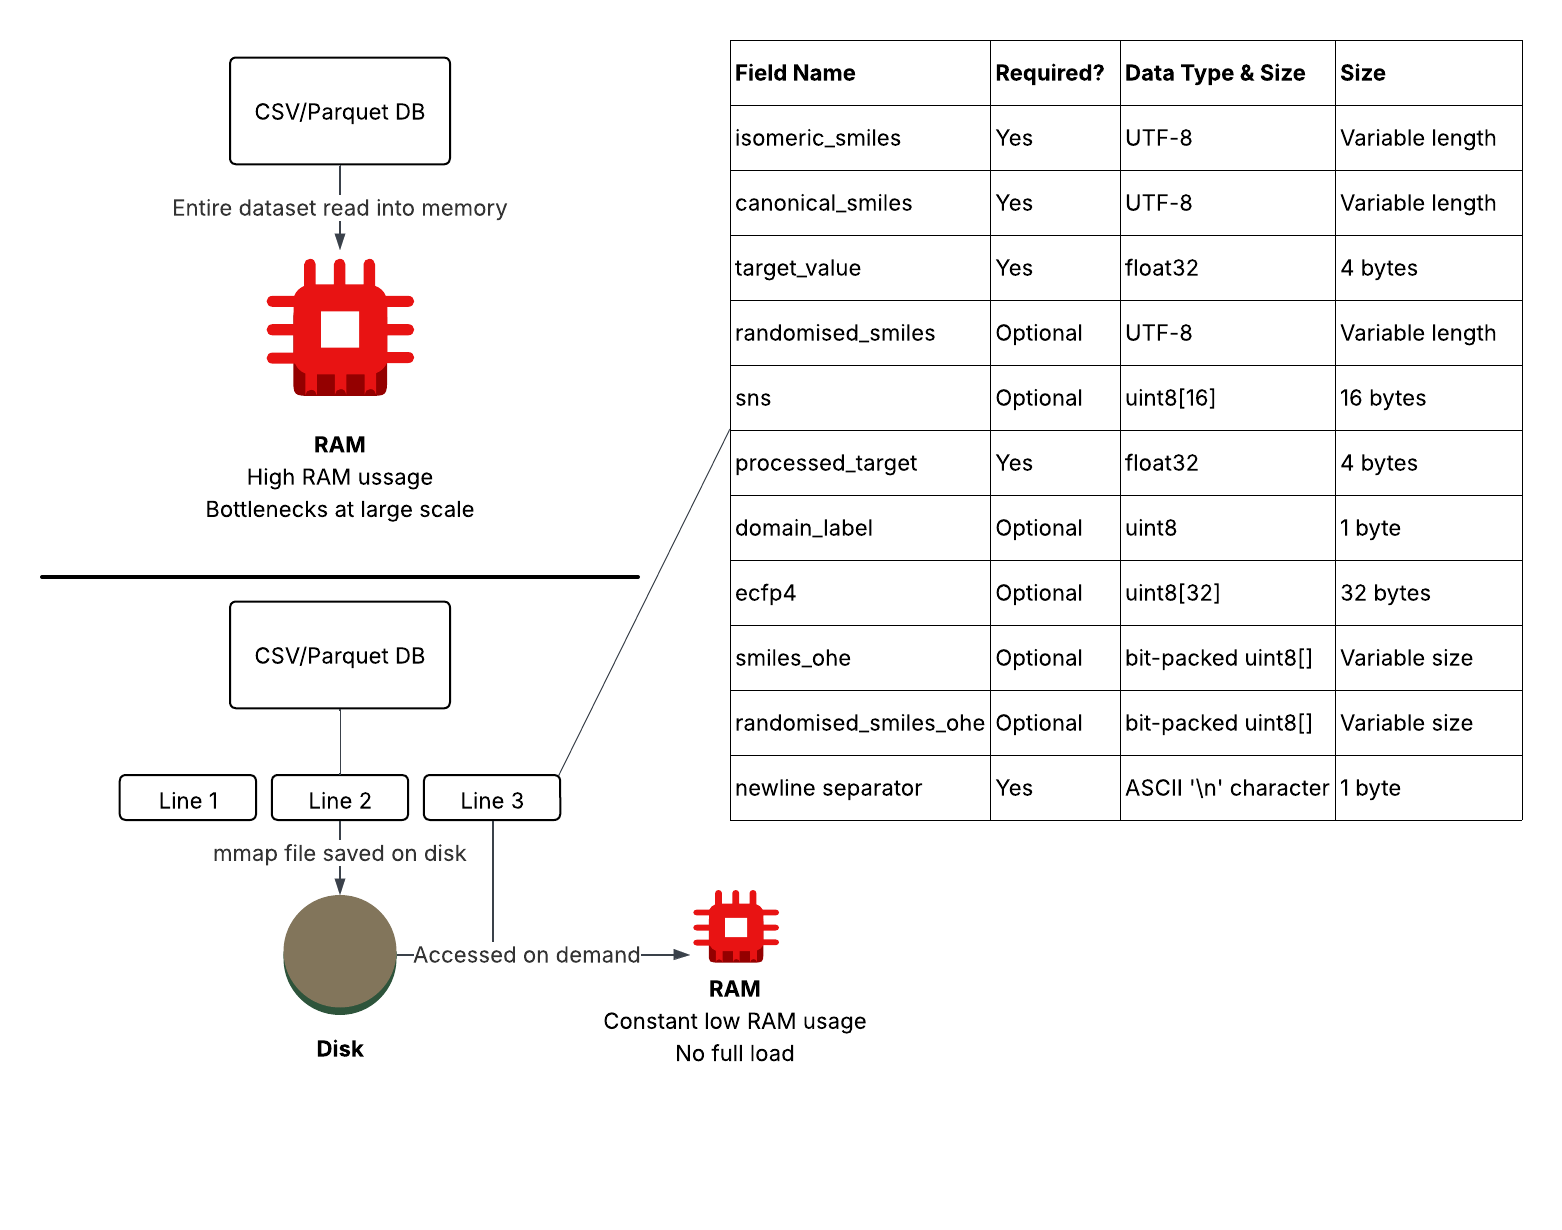
\includegraphics[width=0.95\textwidth,height=0.72\textheight,keepaspectratio]{figure_mmap_structure.png}
    \caption[In-memory and memory-mapped data loading.]{In-memory (top left) and memory-mapped (bottom left) data loading. Memory-mapped loading keeps each molecule as one record of a binary file on disk and reads records into memory on demand. The table on the right lists the fields of one record.}
    \label{fig:fig_mmap}
\end{figure}


\subsection{Uncertainty}
% [notes moved to thesis_notes_moved.md]

Up to this point we have been concerned with how noise affects the predictive performance of QSAR models. However, label noise should also affect the uncertainty these models report. Some models return only a point prediction, while others also return an estimate of uncertainty, either as a predicted distribution or as the spread across an ensemble. Furthermore, some report a single value of uncertainty while others report one that can be decomposed into an aleatoric and an epistemic component \citep{kendall2017}. The aleatoric component describes underlying noise the model associates with the data, while the epistemic component represents the uncertainty within the model's fit. We sought to determine if, as expected, the aleatoric component rises with injected label noise while the epistemic component does not.

For the BNN and VBLL transformations, we took the two components over $T = 100$ stochastic forward
passes \citep{kendall2017}:
\begin{equation}
\hat{u}^2_{\text{ale}}(x) = \frac{1}{T}\sum_{t=1}^{T}\hat{v}_t(x),
\qquad
\hat{u}^2_{\text{epi}}(x) = \frac{1}{T}\sum_{t=1}^{T}\big(\hat{\mu}_t(x) - \bar{\mu}(x)\big)^2 ,
\label{eq:sampling_split}
\end{equation}
where $\hat{\mu}_t(x)$ and $\hat{v}_t(x)$ are the mean and the variance returned for molecule $x$ on
pass $t$, and $\bar{\mu}(x)$ is the mean over passes. Here $\hat{v}_t(x)$ is the predicted observation
noise variance. It varies per molecule in the variance-head and heteroscedastic variants, and is one
number for the whole fit in the VBLL transformation. A full-BNN without a variance head returns no
variance, so its uncertainty is epistemic alone.

% TODO: review, needs manual review
The other models follow the same split. For GPs, the epistemic component is the posterior variance of the latent function and the aleatoric component is the learned observation noise \citep{Rasmussen2005}. Every GP except the heteroscedastic variant learns a single observation-noise variance for the whole fit, so its aleatoric component does not vary between molecules. For QRF models, each leaf holds several training molecules, and the aleatoric component for a molecule is the variance of the training labels in the leaf it falls into, averaged over the trees. The epistemic component is the variance of the leaf means across the trees. NGBoost predicts one variance for each molecule from a single fit, which is aleatoric alone \citep{Duan2020}. In every model, the total uncertainty is the sum of the aleatoric and epistemic components.

% TODO: review, needs manual review
No held-out label carries injected noise, so every comparison against the injected noise was made on
training molecules. Each training set was divided into five folds grouped on Murcko scaffolds, and each
molecule was scored by a refit that excluded its own fold. For NGBoost on QM9, three of the five folds
were scored to limit its cost. No uncertainty was calibrated after fitting. Table~\ref{tab:uncertainty} gives QM9 on PDV rather than on ECFP4, the representation most other tables use, because the QM9 uncertainty runs under censoring were made on PDV only.


\subsection{Evaluation}
% [notes moved to thesis_notes_moved.md]
We computed statistics on the held-out molecules: for QM9 the test split, and for the three assay datasets the held-out fold of the scaffold cross-validation. Different combinations of dataset, model, representation, noise condition, and noise level are examined in each scenario. We used the coefficient of determination ($R^2$) throughout. For molecule $i$, let $y_i$ be the clean label, $\hat{y}_i$ the prediction, $\epsilon_i$ the noise injected into its label and $u_i$ the predicted uncertainty.

% TODO: review, needs manual review
To evaluate the effect of label noise, we tracked predictive performance retention under increasing artificial noise. For each QSAR pairing we recorded $R^2(x)$ at each noise level $x$, and normalized it to obtain the retention ratio $R^2(x)/R^2(0)$. To quantify robustness, we used the normalized area under this retention curve, \aucnorm{} (Equation~\ref{eq:auc_norm}), evaluated using the trapezoidal rule over the seven noise levels, $x \in \{0, 0.2, 0.3, 0.5, 0.75, 1.0, 1.5\}$, in the units of Equation~\ref{eq:dose_matching}. For censoring, the area is taken over the fractions of labels clipped, from 0 to 0.5, so its \aucnorm{} is not on the same axis as the other conditions.

% TODO: review, needs manual review
An \aucnorm{} value near 1 indicates that the QSAR model in question has retained predictive performance with artificial noise, meaning it is more robust to noise. Since we normalize the curve by its own clean-label predictive performance, a model with a low clean $R^2$ has less to lose, so \aucnorm{} is reported beside clean $R^2$. We excluded every QM9 replicate or scaffold fold with a clean $R^2 < 0.3$ from the robustness analysis (Additional file~\ref{app:noise:sec:excluded_configurations}), as performance retention ratios become unstable when the clean-label denominator approaches zero. Under Gaussian noise this removed 58 of 390 scaffold folds on Caco-2, mostly from the Bayesian and VBLL networks on ChemBERTa and MHG-GNN, and 35 of 390 on hERG $K_i$, mostly from the Bayesian and VBLL networks; no LogD fold fell below the threshold. The exclusion applies only to \aucnorm{}, and clean $R^2$ and $R^2$ under noise keep every fold. On QM9 one \aucnorm{} is computed per replicate, and we report the median over the 10 replicates. On the three assay datasets one value is computed per scaffold fold, and the median over the five folds is reported. 

% TODO: review, needs manual review
To test whether a model's robustness follows from its clean predictive performance, we computed Spearman's rank correlation ($\rho$) between clean $R^2$ and \aucnorm{} across the thirteen base models.

% TODO: review, needs manual review
We conducted a separate analysis of variance (ANOVA) for each noise condition to identify the
relative contributions of molecular representation and model architecture to both predictive
performance and noise robustness. For a given metric $y$, either $R^2$ at a noise level of 1.0 (0.75 on Caco-2, whose clean $R^2$ is the lowest of the four datasets and leaves the models less predictive performance to lose) or
\aucnorm:
\begin{equation}
y_{fmjr} = \mu + s_r + \alpha_f + \gamma_{m(f)} + \beta_j + (\alpha\beta)_{fj} + (\gamma\beta)_{m(f)j} + e_{fmjr},
\end{equation}
where $s_r$ represents the effect of replicate $r$, $\alpha_f$ represents the effect of model family $f$, $\gamma_{m(f)}$ represents the effect of model architecture $m$ within its family, $\beta_j$ represents the effect of
molecular representation $j$, $(\alpha\beta)_{fj}$ and $(\gamma\beta)_{m(f)j}$ are the interaction terms, and $e_{fmjr}$ is the
residual. The proportion of variance explained by each term was calculated as the
effect size
\begin{equation}
\eta^2_{\text{term}} = \frac{SS_{\text{term}}}{SS_{\text{total}}},
\end{equation}
using Type I (sequential) sums of squares, entered in the order replicate, model family, model architecture within family, molecular
representation, interaction. The 10 QM9 replicates provide the residual; on the three assay datasets the five scaffold folds take the place of the replicates. The clean fit is made once per replicate and every noise condition starts from it, so the decomposition of clean $R^2$ has no noise condition. The uncertainty on each share is the 95\% interval of $\eta^2$ over 1,000 bootstrap resamples of whole replicates, and these intervals are given in Additional file~\ref{app:noise:sec:variance_intervals}. These shares describe the models and representations tested here, not the choice of model or representation in general. 

ANOVA relies on the assumption that observations both within and across groups are independent. Two features of this study break that assumption. First, each QM9 replicate uses the same data split and the same noise draw for every model and representation, so observations from one replicate are not independent of each other; we therefore entered the replicate as a block. Second, across the whole set of models in this study, some pairs produced similar predictions that are not independent, so a method present in several near-identical versions would count several times toward the share of model architecture. To handle this issue, we grouped the models into families. We considered grouping pairs of models that share a method or an architecture, and compared each pair on clean $R^2$ and on \aucnorm{} under the three noise conditions run on every representation, separately on each of the six representations, which gives 24 comparisons per pair. A pair was grouped when the mean difference between the two models was smaller than their standard deviation across replicates in at least two thirds of these comparisons (Additional file~\ref{app:noise:sec:model_redundancy}). Five families met this criterion: RF with QRF (16 of 24), XGBoost with LightGBM (23 of 24), NN-$\alpha$ with BNN-$\alpha$ (20 of 24), NN-$\beta$ with BNN-$\beta$ (18 of 24), and VBLL-$\alpha$ with VBLL-$\beta$ (20 of 24). VBLL did not group with the plain or Bayesian network of its own architecture (4 to 10 of 24), as its clean $R^2$ was lower by 0.02 to 0.09, and NGBoost did not group with XGBoost or LightGBM (2 and 3 of 24). The two architectures of the plain networks, and of the Bayesian networks, also met the criterion (18 and 17 of 24); we grouped by architecture instead, which the evidence supports equally well. The thirteen base models therefore form eight families. Within these families, the differences between models accounted for at most 1.0\% of the variance in any outcome and noise condition on QM9, and up to 15.1\% of predictive performance on clean labels on the three assay datasets. We also ran Tukey's honestly significant difference test between the members of each family, separately for each representation (Additional file~\ref{app:noise:sec:tukey_within_families}). With 10 replicates it detects differences smaller than the variation between replicates, so we report it beside the size of each difference rather than use it to form the families.

% TODO: review, needs manual review
Across representations, we considered grouping Sort \& Slice with the ECFP4 fingerprint, as both encode overlapping circular substructure information. The grouping criterion held for none of the 13 base models on clean $R^2$, so all six representations were kept as separate levels (Additional file~\ref{app:noise:sec:representation_redundancy}).

% TODO: review, needs manual review
To assess the interaction between uncertainty estimation and label noise, we carried out four analyses. The first tested whether uncertainty rises with label noise, as measured by the mean $u_i$ over held-out molecules at the highest noise level
divided by its value with no added noise, in each fold. The second pertains to models that report separate aleatoric and epistemic components. We divided the increase of mean epistemic uncertainty between the highest level of noise and clean labels by the increase in the mean aleatoric component to determine how each responds to label noise. A ratio near 0 means the added noise was attributed to the labels while a ratio of 1 or above means the epistemic component grew as much or more. Table~\ref{tab:uncertainty} also gives each component's slope against the noise level, a least-squares line through the mean uncertainty at each level, in the label's units per unit of added noise. A component that is a single number per fit is given no slope, because a slope through a constant describes the fit rather than the molecules. We also compared the mean aleatoric component with the standard deviation of the injected noise. The third tested whether per-sample uncertainty values track injected label noise, as measured by the Spearman correlation between $u_i$ and $|\epsilon_i|$ over out-of-fold training molecules, per fold and per noise level. We also report the Spearman correlation between $u_i$ and the absolute error of the prediction. The fourth tested whether dividing a molecule's out-of-fold absolute error by $u_i$ ranks the corrupted labels better than the error alone. We took the 10\% of molecules with the largest $|\epsilon_i|$ as corrupted and scored each ranking by its AUC, the probability that a corrupted molecule is ranked above one that is not, and we report $\Delta$AUC, the AUC of the error divided by $u_i$ minus the AUC of the error alone. $\Delta$AUC is computed in each fold and the median over folds is reported, so it need not equal the difference of the two AUC columns' medians. No interval was computed for it, so it gives a direction and not a significance.


\section{Variance Decomposition}
% [notes moved to thesis_notes_moved.md]

% TODO: review, needs manual review
Considering the two main components of a QSAR model, the molecular representation and the model architecture, we sought to understand how each contributes to both predictive performance and noise robustness. ANOVA decomposition divides the variance between model family, model architecture within its family, molecular representation, the pairing of the two, the replicate, and a residual. We ran this decomposition for Gaussian noise, the usual assumption, as well as the two conditions that act on scaffold families, grouped-wider and grouped-shifted (Figure~\ref{fig:variance}, Table~\ref{tab:variance}). For predictive performance measured in $R^2$ at a noise level of 1.0, model family and molecular representation account for comparable shares of the variance, 26.6\% and 29.0\% under Gaussian noise. However, for noise robustness, quantified by the normalized area under the $R^2$ retention curve (\aucnorm; higher values indicate greater robustness), model family accounts for 47.2\% of the variance while molecular representation accounts for 8.1\%. This pattern is observed across noise conditions. However, the interaction term between model architecture and molecular representation is slightly more influential with noise robustness than with predictive performance, 19.9\% against 14.2\%, though it is on par with the residual. Some models may depend on particular representations more strongly once the labels are noisy.

\begin{figure}[!htbp]
\centering
\includegraphics[width=\textwidth,height=0.72\textheight,keepaspectratio]{F2_variance_decomposition.png}
\caption[Variance decomposition of robustness and predictive performance on QM9.]{Share of the variance in each outcome explained by model family, model architecture within family, molecular representation, their pairing, the replicate, and the residual, on the QM9 HOMO--LUMO gap. a) Robustness, as \aucnorm; b) predictive performance, as $R^2$ at a noise level of 1.0, one spread of the clean training labels. The bottom axis is the noise condition, the side axis the share of variance. Whiskers are 95\% bootstrap intervals over replicates.}
\label{fig:variance}
\end{figure}

Comparing the decomposition before and after noise is added shows where model family matters (Table~\ref{tab:three_outcomes_qm9}, Figure~\ref{fig:three_outcomes}). For predictive performance, noise changes the division of the variance only a little. Representation explains about the same share of $R^2$ with and without noise, model family loses some of its share, and the replicate and the residual together take more. Robustness divides the variance differently. Representation explains 8.1\% of the variance in \aucnorm, against 31.1\% of clean $R^2$, while model family rises to 47.2\%. The replicate nearly disappears from \aucnorm, likely because each replicate's curve is divided by that replicate's own clean $R^2$, so a difficult split lowers both and cancels out.

\begin{table}[!htbp]
\centering
\small
\begin{adjustbox}{max width=\textwidth,max totalheight=0.78\textheight}
\begin{tabular}{lccc}
\toprule
Term & Clean $R^2$ & $R^2$ at noise level 1.0, Gaussian & \aucnorm, Gaussian \\
\midrule
Model family & 35.4 & 26.6 & 47.2 \\
Representation & 31.1 & 29.0 & 8.1 \\
Model $\times$ representation & 12.1 & 14.2 & 19.9 \\
Replicate & 10.6 & 13.4 & 1.7 \\
Residual & 10.2 & 16.0 & 22.6 \\
\bottomrule
\end{tabular}
\end{adjustbox}
\caption[Variance shares before and after Gaussian noise on QM9.]{Share of the variance (\%) in each outcome explained by each term, on the QM9 HOMO--LUMO gap, before and after Gaussian noise is added. Clean $R^2$ is predictive performance with no noise added; the second column is $R^2$ at the noise level named in its header; \aucnorm{} is robustness. Model within family, the remaining term, is left out, so a column does not sum to 100\%.}
\label{tab:three_outcomes_qm9}
\end{table}

% TODO: this figure shows the same numbers as Table tab:three_outcomes_qm9 (both are in the main text of the NoiseInject manuscript); keep one of the two if pages are short.
\begin{figure}[!htbp]
\centering
\includegraphics[width=\textwidth,height=0.72\textheight,keepaspectratio]{F2c_three_outcomes.png}
\caption[Variance shares of clean performance, noisy performance and robustness on QM9.]{Share of the variance in each outcome explained by each term on the QM9 HOMO--LUMO gap, in three groups: predictive performance on clean labels, predictive performance at a noise level of 1.0 under Gaussian noise, and robustness (\aucnorm) under Gaussian noise. One bar per term. Whiskers are 95\% bootstrap intervals over replicates.}
\label{fig:three_outcomes}
\end{figure}

% TODO: review, needs manual review
Under grouped-shifted noise the pattern changes, because predictive performance varies widely between replicates, which gives the replicate a larger share. We find that 28.4\% of the variance in \aucnorm{} and 51.0\% of the variance in $R^2$ are due to the replicate, with model family falling to 32.7\% and 8.4\%. The offset applied to each scaffold family may therefore account for more of the variance in both $R^2$ and \aucnorm.

\begin{table}[!htbp]
\centering
\small
\begin{adjustbox}{max width=\textwidth,max totalheight=0.78\textheight}
\begin{tabular}{llcccccc}
\toprule
Condition & Outcome & Replicate $\eta^2$ (\%) & Model family $\eta^2$ (\%) & Model within family $\eta^2$ (\%) & Representation $\eta^2$ (\%) & Interaction $\eta^2$ (\%) & Residual $\eta^2$ (\%) \\
\midrule
None (clean labels) & Performance (clean $R^2$) & 10.6 & 35.4 & 0.6 & 31.1 & 12.1 & 10.2 \\
Gaussian & Robustness (\aucnorm) & 1.7 & 47.2 & 0.6 & 8.1 & 19.9 & 22.6 \\
Grouped-shifted & Robustness (\aucnorm) & 28.4 & 32.7 & 1.0 & 7.0 & 7.2 & 23.7 \\
Grouped-wider & Robustness (\aucnorm) & 1.7 & 46.3 & 0.3 & 7.9 & 18.5 & 25.3 \\
Gaussian & Performance ($R^2$ at level 1.0) & 13.4 & 26.6 & 0.8 & 29.0 & 14.2 & 16.0 \\
Grouped-shifted & Performance ($R^2$ at level 1.0) & 51.0 & 8.4 & 0.4 & 10.3 & 6.2 & 23.7 \\
Grouped-wider & Performance ($R^2$ at level 1.0) & 12.7 & 33.0 & 0.4 & 25.7 & 13.1 & 15.1 \\
\bottomrule
\end{tabular}
\end{adjustbox}
\caption[Variance decomposition by noise condition on QM9.]{Share of the variance in each outcome explained by the replicate, model family, model architecture within family, molecular representation, their pairing and the residual, on the QM9 HOMO--LUMO gap. Robustness is \aucnorm; performance is $R^2$ at a noise level of 1.0.}
\label{tab:variance}
\end{table}

\section{Predictive Performance and Noise Robustness}
% [notes moved to thesis_notes_moved.md]

% TODO: review, needs manual review
The variance decomposition tells us what aspect of QSAR modeling affects predictive performance and robustness; however, it does not tell us about the characteristics of individual models. Every model's performance degrades as the labels get increasingly corrupted with noise (Figure~\ref{fig:curves}). Performance changes little until the artificial noise reaches about half the spread of the clean training labels, and then it begins to drop. The rate at which it drops and the amount of predictive performance retained are not necessarily correlated with the model's predictive performance on clean labels. Across the thirteen base models under Gaussian noise on ECFP4, clean $R^2$ and \aucnorm{} are unrelated, at a Spearman correlation of $-0.16$ ($p = 0.61$). If anything, the lower a model's predictive performance on clean labels, the less it has to lose as the labels get noisier.

\begin{figure}[!htbp]
\centering
\includegraphics[width=\textwidth,height=0.72\textheight,keepaspectratio]{F4a_models_under_noise.png}
\caption[Predictive performance against Gaussian label noise on QM9.]{Predictive performance against label noise on the QM9 HOMO--LUMO gap under Gaussian noise, for the eight base models with the highest \aucnorm{} on ECFP4. a) ECFP4; b) PDV, drawn for the same eight models. Bottom axis: the noise level, as a fraction of the spread of the clean training labels. Side axis: $R^2$ on held-out molecules, as the median over 10 replicates. The dashed vertical line marks the noise level of 1.0 at which $R^2$ is reported.}
\label{fig:curves}
\end{figure}

The link between predictive performance and noise robustness can be examined by model family (Figure~\ref{fig:decoupling}, Table~\ref{tab:robustness}). The forests, XGBoost, LightGBM, SVM and GP all retain relatively high predictive performance on clean labels while maintaining relatively strong robustness to noise. NN-$\beta$ and BNN-$\beta$ are among the highest in predictive performance on clean labels, and the four plain and Bayesian networks are the four least robust. The two variational networks sit between these groups, with lower predictive performance on clean labels and middling noise robustness. Standard feed-forward networks can make strong predictions under clean labels; however, they are not a safe bet under noisy ones.

\begin{figure}[!htbp]
\centering
\includegraphics[width=\textwidth,height=0.72\textheight,keepaspectratio]{R16_decoupling_ecfp4.png}
\caption[Clean predictive performance against robustness on QM9.]{Predictive performance on clean labels against robustness, on the QM9 HOMO--LUMO gap on ECFP4, under a) Gaussian and b) grouped-shifted noise. One point per base model. Bottom axis: $R^2$ with no noise added to the training labels. Side axis: \aucnorm, on one scale across both panels.}
\label{fig:decoupling}
\end{figure}

% TODO: the four plain and Bayesian networks' grouped columns and clean R^2 will move once their clean scores are fixed (carried over from the NoiseInject manuscript).
\begin{table}[!htbp]
\centering
\small
\begin{adjustbox}{max width=\textwidth,max totalheight=0.78\textheight}
\begin{tabular}{lcccccccc}
\toprule
Model & Clean $R^2$ & Gaussian & Grouped-wider & Grouped-shifted & Censoring & Student-$t$ ($\nu$=5) & Outlier (10\%) & Laplace \\
\midrule
RF & 0.832 & 0.963 & 0.967 & 0.937 & 0.817 & 0.966 & 0.969 & 0.967 \\
QRF & 0.830 & 0.956 & 0.973 & 0.928 & --- & --- & --- & --- \\
XGBoost & 0.835 & 0.946 & 0.940 & 0.918 & --- & --- & --- & --- \\
LightGBM & 0.845 & 0.938 & 0.937 & 0.908 & --- & --- & --- & --- \\
NGBoost & 0.706 & 0.979 & 0.953 & 0.933 & --- & 0.969 & 0.963 & 0.966 \\
SVM & 0.844 & 0.937 & 0.955 & 0.908 & --- & 0.945 & 0.951 & 0.951 \\
GP & 0.839 & 0.938 & 0.939 & 0.905 & --- & 0.940 & 0.938 & 0.936 \\
NN-$\alpha$ & 0.794 & 0.910 & 0.910 & 0.857 & --- & --- & --- & --- \\
BNN-$\alpha$ & 0.820 & 0.887 & 0.886 & 0.853 & --- & --- & --- & --- \\
VBLL-$\alpha$ & 0.772 & 0.926 & 0.927 & 0.920 & --- & --- & --- & --- \\
NN-$\beta$ & 0.842 & 0.872 & 0.881 & 0.848 & --- & --- & --- & --- \\
BNN-$\beta$ & 0.839 & 0.871 & 0.866 & 0.840 & --- & --- & --- & --- \\
VBLL-$\beta$ & 0.754 & 0.924 & 0.925 & 0.916 & --- & --- & --- & --- \\
\bottomrule
\end{tabular}
\end{adjustbox}
% TODO: review, needs manual review
\caption[Robustness of each base model under each noise condition on QM9.]{Robustness (\aucnorm) of each base model under each noise condition on the QM9 HOMO--LUMO gap with ECFP4, with clean $R^2$ in the first column. A dash is a pairing the condition was not run on. Values are medians over 10 replicates.}
\label{tab:robustness}
\end{table}

% TODO: review, needs manual review
NGBoost is a standout case in the sense that it is highly dependent on its paired molecular representation. Under Gaussian noise it has the highest \aucnorm{} on every one of the six representations, yet also the lowest predictive performance on clean labels on four of the six representations. Its high robustness is partly due to the fact that a model that starts from low predictive performance does not have as much to lose. It also maintains shallow robustness curves across representations. On ECFP4, NGBoost's predictive performance ranks lowest up to a noise level of 0.75 and stays in the lower half at every noise level. However, on PDV it starts second lowest and ends highest, surpassing the other models between noise levels 1.0 and 1.5. So when paired with the right features, NGBoost has the potential to make better predictions under higher quantities of label noise. Under grouped-shifted noise, RF has higher \aucnorm{} values than NGBoost on ECFP4, Avalon and ChemBERTa. Even then, NGBoost reports the highest noise robustness for PDV, MHG-GNN and Sort \& Slice. While NGBoost on PDV performs well under higher label noise, LightGBM performs well under smaller quantities of noise. Its performance drops sharply after a noise level of 1.0.

% TODO: review, needs manual review
The choice of representation can affect noise robustness, but how much depends on the model family (Figure~\ref{fig:grid}; the same grid under grouped-wider noise is in Additional file~\ref{app:noise:sec:grouped_wider_grid}). All of the neural networks span a wider range of \aucnorm{} across the six representations than any of the other models, 0.037 to 0.069 against at most 0.030. Between ECFP4 and PDV under Gaussian noise, the four plain and Bayesian networks differ by between 0.037 and 0.065 of \aucnorm, while no tree or kernel model shifts by more than 0.011. This does not hold for every network; the two variational networks move by 0.009 and 0.019. So while molecular representation is not the primary factor in what makes a model robust to noise, the choice of which molecular representation to use matters with certain models, particularly neural networks.

\begin{figure}[!htbp]
\centering
\includegraphics[width=\textwidth,height=0.72\textheight,keepaspectratio]{F3_model_by_representation.png}
\caption[Robustness of each base model on each representation on QM9.]{Robustness (\aucnorm) of the thirteen base models on the QM9 HOMO--LUMO gap under a) Gaussian and b) grouped-shifted noise. Rows are models, ordered by family, and columns the six representations. Color is fixed across both panels, its bright end the higher \aucnorm. Values are medians over 10 replicates.}
\label{fig:grid}
\end{figure}

\section{Artificial Noise Conditions}
% [notes moved to thesis_notes_moved.md]

% TODO: review, needs manual review
Many studies involving experimental label noise rely on the assumption that noise can be modeled by a Gaussian distribution. We decided to vary the distribution from which noise is drawn, as well as the way in which it is injected into specific labels. Five of the seven conditions draw each label's error on its own, so the error is random. Grouped-shifted gives a whole scaffold family a shared offset, and censoring pulls every label above a limit down to that limit, so in both the error is systematic. Every condition except censoring adds the same expected amount of noise at a given noise level (Section~\ref{sec:noise_injection}), so a difference between two conditions is a difference in pattern rather than amount. Censoring could not be held to a set amount, as its levels count the fraction of labels clipped.

We compare Gaussian noise on the HOMO--LUMO gap to Laplace, Student-$t$ and outlier noise in Figure~\ref{fig:deep}. The shape of the distribution from which the noise was drawn made little difference. SVM reported higher \aucnorm{} values on non-Gaussian label noise, 0.937 under Gaussian noise against 0.947, 0.952 and 0.955 under Student-$t$, outlier and Laplace noise on PDV (the ECFP4 values are in Table~\ref{tab:robustness}), while NGBoost lost \aucnorm{} under every one. NGBoost's relatively stronger performance under Gaussian noise makes sense, as it fits a per-molecule scale under a Gaussian likelihood, which the other distributions violate. No single change exceeds the spread across that pairing's ten replicates on QM9. These results coincide with \citet{Heid2023}, who found no difference between error distributions drawn at a matched mean and standard deviation.

\begin{figure}[!htbp]
\centering
\includegraphics[width=\textwidth,height=0.72\textheight,keepaspectratio]{R19_deep_conditions_qm9.png}
% TODO: review, needs manual review
\caption[Robustness under every noise condition on a subset of models on QM9.]{Robustness (\aucnorm) under every noise condition for the eight models run under Laplace, Student-$t$ and outlier noise, on the QM9 HOMO--LUMO gap. a) ECFP4; b) PDV; c) ChemBERTa. Rows are models and columns noise conditions, with Gaussian on the left. Values are medians over 10 replicates, on one color scale across all panels. A gray square marks a pairing that was not run.}
\label{fig:deep}
\end{figure}

% TODO: review, needs manual review
The Gaussian distribution stands in well for the other noise shapes, but not for systematic noise. Relative to Gaussian, grouped-shifted noise lowered \aucnorm{} across all models and representations (Table~\ref{tab:condition_cost}). The models struggle when the molecules of a scaffold family share an offset rather than each receiving an independent error. For RF on ECFP4, the grouped-shifted curve separates from those of the other conditions from a noise level of 0.75 (Figure~\ref{fig:conditions}). The variational networks retained the most predictive performance, while the plain, deterministic NNs lost the most. BNN-$\alpha$ lost less \aucnorm{} between Gaussian and grouped-shifted noise than NN-$\alpha$ on every representation except PDV, while BNN-$\beta$ lost less than NN-$\beta$ by more than 0.01 only on MHG-GNN and PDV (Table~\ref{tab:condition_cost}). Grouped-wider noise changed no model beyond its replicate spread except QRF on Avalon and MHG-GNN, whose \aucnorm{} rose under this condition. Censoring gave \aucnorm{} values 0.12 to 0.18 below those under Gaussian noise for the same models, although its noise level counts the fraction of labels clipped and so is not the same axis (Figure~\ref{fig:deep}).

\begin{table}[!htbp]
\centering
\small
\begin{adjustbox}{max width=\textwidth,max totalheight=0.78\textheight}
\begin{tabular}{lcccccccc}
\toprule
Model & ECFP4 & PDV & MHG-GNN & Avalon & ChemBERTa & Sort \& Slice & Replicate spread & Beats it on \\
\midrule
RF & -0.025 & -0.024 & -0.025 & -0.038 & -0.025 & -0.028 & 0.013--0.022 & 6 of 6 \\
QRF & -0.027 & -0.027 & -0.032 & -0.042 & -0.027 & -0.038 & 0.016--0.031 & 5 of 6 \\
XGBoost & -0.028 & -0.039 & -0.035 & -0.052 & -0.030 & -0.025 & 0.016--0.039 & 5 of 6 \\
LightGBM & -0.030 & -0.037 & -0.037 & -0.058 & -0.028 & -0.037 & 0.016--0.033 & 5 of 6 \\
NGBoost & -0.046 & -0.030 & -0.039 & -0.062 & -0.041 & -0.039 & 0.019--0.041 & 6 of 6 \\
SVM & -0.029 & -0.045 & -0.034 & -0.053 & -0.040 & -0.038 & 0.022--0.043 & 5 of 6 \\
GP & -0.034 & -0.048 & -0.040 & -0.054 & -0.045 & -0.041 & 0.025--0.038 & 6 of 6 \\
NN-$\alpha$ & -0.053 & -0.051 & -0.060 & -0.115 & -0.044 & -0.053 & 0.025--0.055 & 4 of 6 \\
BNN-$\alpha$ & -0.034 & -0.053 & -0.034 & -0.073 & -0.039 & -0.025 & 0.027--0.075 & 2 of 6 \\
VBLL-$\alpha$ & -0.006 & -0.014 & -0.020 & -0.005 & -0.007 & -0.013 & 0.029--0.047 & 0 of 6 \\
NN-$\beta$ & -0.024 & -0.080 & -0.052 & -0.076 & -0.047 & -0.045 & 0.032--0.048 & 4 of 6 \\
BNN-$\beta$ & -0.030 & -0.050 & -0.019 & -0.075 & -0.055 & -0.041 & 0.032--0.180 & 2 of 6 \\
VBLL-$\beta$ & -0.007 & -0.028 & -0.033 & -0.010 & -0.028 & -0.009 & 0.030--0.066 & 0 of 6 \\
\bottomrule
\end{tabular}
\end{adjustbox}
\caption[Change in robustness from Gaussian to grouped-shifted noise on QM9.]{The change in \aucnorm{} from Gaussian to grouped-shifted noise on the QM9 HOMO--LUMO gap, for each base model on each representation; negative is a loss. The replicate spread is the highest minus the lowest \aucnorm{} across a pairing's 10 replicates under Gaussian noise, given as its range over the representations. The last column counts the representations on which the loss exceeds that spread.}
\label{tab:condition_cost}
\end{table}

\begin{figure}[!htbp]
\centering
\includegraphics[width=\textwidth,height=0.72\textheight,keepaspectratio]{F4b_rf_across_noise_conditions.png}
\caption[Random forest under each noise condition on QM9.]{Predictive performance of the random forest under each noise condition, one line per condition, on the QM9 HOMO--LUMO gap on ECFP4. The bottom axis is the noise added to the training labels, as a fraction of their clean spread, and the side axis median held-out $R^2$ over 10 replicates. Censoring is not drawn.}
\label{fig:conditions}
\end{figure}

% TODO: review, needs manual review
While we established that the choice of representation has only a minor impact on noise robustness, representations do seem to perform better or worse under different noise conditions. When compared to Gaussian noise, under grouped-shifted noise NGBoost went from performing best on Avalon to PDV, SVM went from ChemBERTa to ECFP4 and BNN-$\alpha$ from PDV to MHG-GNN. There is no single best representation for \aucnorm; rather, it depends on the underlying data, including both the samples themselves and the underlying label noise. A representation chosen under one assumption about the noise is therefore not necessarily the best under another.

% TODO: review, needs manual review
Most of these observations are made at the upper end of the noise range. With ECFP4, six of the seven most robust models start within 0.015 of one another in $R^2$ for clean labels, stay together up to a noise level of 0.5 and separate only above 1.0, finishing between 0.692 for LightGBM and 0.741 for RF (Figure~\ref{fig:curves}). We ranked the models by predictive performance at each noise level within each replicate and took the median rank over replicates. Of the thirteen base models, RF started ranked seventh, but by level 1.0 it was ranked first. SVM, on the other hand, falls from first to fifth (Figure~\ref{fig:rank_level}). Because \aucnorm{} weights the whole range from 0 to 1.5 equally, and the first half of it separates little, it has the potential to understate just how much the pattern of the noise costs. However, choosing to look at performance at a set level has its drawbacks, as the ranks shift at a different pace between noise conditions.

\begin{figure}[!htbp]
\centering
\includegraphics[width=\textwidth,height=0.36\textheight,keepaspectratio]{R15_rank_against_level_ecfp4_gaussian.png}\\[4pt]
\includegraphics[width=\textwidth,height=0.36\textheight,keepaspectratio]{R15_rank_against_level_ecfp4_grouped_shifted.png}
\caption[Rank of each base model at each noise level on QM9.]{Rank of each base model for predictive performance at each noise level, on the QM9 HOMO--LUMO gap on ECFP4, under a) Gaussian and b) grouped-shifted noise. The bottom axis is the noise level and the side axis the rank among the thirteen base models, 1 the highest predictive performance. Each point is the median rank over 10 replicates, so ties appear as half ranks.}
\label{fig:rank_level}
\end{figure}

\section{Robustness on the Three Assay Datasets}
% [notes moved to thesis_notes_moved.md]

% TODO: review, needs manual review
So far, we have only discussed results on the HOMO--LUMO gap from QM9, a computed property whose labels carry negligible measurement noise. We repeated these experiments on three experimentally obtained datasets, LogD, Caco-2 \citep{openadmet} and hERG $K_i$ \citep{Zdrazil2023}, replicating our process of adding artificial noise. Unlike QM9, the experimental endpoints carry their own measurement noise in both training and test labels; the injected artificial noise therefore adds on top of an unknown noise floor. Repeat measurements of the same compound disagree by about 0.54 log units for p$K_i$ \citep{Kalliokoski2013, Kramer2012}. The hERG $K_i$ labels have a spread of 0.915 log units, so a noise level of 0.6 of that spread is about one unit of that estimated laboratory error. Each model's \aucnorm{} under the three noise conditions run on every model is given with its clean $R^2$ beside it (Figure~\ref{fig:assay}), and the same values for the six variant models are in Additional file~\ref{app:noise:sec:variant_models_assay}. Censoring is left out of Figure~\ref{fig:assay}, because on the assay datasets its \aucnorm{} was computed for only five pairings of model and representation and so cannot rank the models. The color range in Figure~\ref{fig:assay} differs in span from the range in Figure~\ref{fig:grid} by a factor of three, so color cannot be compared between the two figures.

% TODO: review, needs manual review
Tables~\ref{tab:three_outcomes_logd}, \ref{tab:three_outcomes_caco2} and~\ref{tab:three_outcomes_herg} repeat the QM9 comparison on the three assay datasets. Figure~\ref{fig:variance_clean} and Table~\ref{tab:variance_clean} give the clean decomposition on all four datasets; its QM9 row is the clean row of Table~\ref{tab:variance}. On every dataset, representation explains about the same share of predictive performance with and without noise and a smaller share of robustness than of predictive performance, while model family explains the largest share of robustness. Noise raises the share of the replicate and the residual in predictive performance on every dataset. On Caco-2 and hERG $K_i$ the replicate, which on these datasets is one of five scaffold folds, is the largest share of predictive performance before and after noise is added, but falls well below model family for robustness. Across Gaussian, grouped-wider and grouped-shifted noise on all four datasets, representation explains at most 11.2\% of the variance in \aucnorm{}, on LogD under grouped-shifted noise (Additional file~\ref{app:noise:sec:variance_intervals}).

\begin{table}[!htbp]
\centering
\small
\begin{adjustbox}{max width=\textwidth,max totalheight=0.78\textheight}
\begin{tabular}{lccc}
\toprule
Term & Clean $R^2$ & $R^2$ at noise level 1.0, Gaussian & \aucnorm, Gaussian \\
\midrule
Model family & 60.2 & 59.6 & 58.0 \\
Representation & 16.8 & 14.8 & 7.1 \\
Model $\times$ representation & 9.5 & 9.3 & 12.2 \\
Replicate & 3.3 & 4.5 & 1.3 \\
Residual & 3.6 & 6.3 & 16.3 \\
\bottomrule
\end{tabular}
\end{adjustbox}
\caption[Variance shares before and after Gaussian noise on LogD.]{Share of the variance (\%) in each outcome explained by each term, on LogD, before and after Gaussian noise is added. Clean $R^2$ is predictive performance with no noise added; the second column is $R^2$ at the noise level named in its header; \aucnorm{} is robustness. Model within family, the remaining term, is left out, so a column does not sum to 100\%.}
\label{tab:three_outcomes_logd}
\end{table}

\begin{table}[!htbp]
\centering
\small
\begin{adjustbox}{max width=\textwidth,max totalheight=0.78\textheight}
\begin{tabular}{lccc}
\toprule
Term & Clean $R^2$ & $R^2$ at noise level 0.75, Gaussian & \aucnorm, Gaussian \\
\midrule
Model family & 22.8 & 11.4 & 43.2 \\
Representation & 9.9 & 9.7 & 3.1 \\
Model $\times$ representation & 8.9 & 6.6 & 9.4 \\
Replicate & 38.7 & 56.0 & 18.6 \\
Residual & 6.2 & 10.5 & 20.8 \\
\bottomrule
\end{tabular}
\end{adjustbox}
\caption[Variance shares before and after Gaussian noise on Caco-2.]{Share of the variance (\%) in each outcome explained by each term, on Caco-2, before and after Gaussian noise is added. Clean $R^2$ is predictive performance with no noise added; the second column is $R^2$ at the noise level named in its header; \aucnorm{} is robustness. Model within family, the remaining term, is left out, so a column does not sum to 100\%.}
\label{tab:three_outcomes_caco2}
\end{table}

\begin{table}[!htbp]
\centering
\small
\begin{adjustbox}{max width=\textwidth,max totalheight=0.78\textheight}
\begin{tabular}{lccc}
\toprule
Term & Clean $R^2$ & $R^2$ at noise level 1.0, Gaussian & \aucnorm, Gaussian \\
\midrule
Model family & 18.4 & 22.5 & 47.9 \\
Representation & 6.7 & 5.6 & 0.8 \\
Model $\times$ representation & 14.3 & 7.0 & 13.0 \\
Replicate & 28.1 & 39.4 & 5.0 \\
Residual & 17.5 & 23.5 & 28.0 \\
\bottomrule
\end{tabular}
\end{adjustbox}
\caption[Variance shares before and after Gaussian noise on hERG $K_i$.]{Share of the variance (\%) in each outcome explained by each term, on hERG $K_i$, before and after Gaussian noise is added. Clean $R^2$ is predictive performance with no noise added; the second column is $R^2$ at the noise level named in its header; \aucnorm{} is robustness. Model within family, the remaining term, is left out, so a column does not sum to 100\%.}
\label{tab:three_outcomes_herg}
\end{table}

\begin{figure}[!htbp]
\centering
\includegraphics[width=\textwidth,height=0.72\textheight,keepaspectratio]{F2b_clean_decomposition.png}
\caption[Variance decomposition of clean predictive performance on all four datasets.]{Share of the variance in predictive performance on clean labels explained by model family, model architecture within family, molecular representation, their pairing, the replicate, and the residual, on all four datasets. Predictive performance is $R^2$ on held-out molecules with no noise added to the training labels. The bottom axis is the dataset, the side axis the share of variance; the six shares within a dataset sum to 100\%. Whiskers are 95\% bootstrap intervals over replicates, which on each assay dataset are the five scaffold folds.}
\label{fig:variance_clean}
\end{figure}

\begin{table}[!htbp]
\centering
\small
\begin{adjustbox}{max width=\textwidth,max totalheight=0.78\textheight}
\begin{tabular}{lcccccc}
\toprule
Dataset & Replicate $\eta^2$ (\%) & Model family $\eta^2$ (\%) & Model within family $\eta^2$ (\%) & Representation $\eta^2$ (\%) & Interaction $\eta^2$ (\%) & Residual $\eta^2$ (\%) \\
\midrule
Caco-2 & 38.7 & 22.8 & 13.4 & 9.9 & 8.9 & 6.2 \\
hERG $K_i$ & 28.1 & 18.4 & 15.1 & 6.7 & 14.3 & 17.5 \\
LogD & 3.3 & 60.2 & 6.7 & 16.8 & 9.5 & 3.6 \\
QM9 (HOMO--LUMO gap) & 10.6 & 35.4 & 0.6 & 31.1 & 12.1 & 10.2 \\
\bottomrule
\end{tabular}
\end{adjustbox}
\caption[Variance decomposition of clean predictive performance by dataset.]{Share of the variance in predictive performance on clean labels explained by the replicate, model family, model architecture within family, molecular representation, their pairing and the residual, one row per dataset. On each assay dataset a replicate is one of five scaffold folds.}
\label{tab:variance_clean}
\end{table}

% TODO: review, needs manual review
As on QM9, the noise distribution changes the \aucnorm{} of most models little (Table~\ref{tab:assay_shape}). Laplace, Student-$t$ and outlier noise were run on seven models, RF, the two GPs, SVM, NGBoost, BNN-$\alpha$ (var.\ head) and VBLL-$\beta$ (het.), on ECFP4, PDV and ChemBERTa. Each change below is measured from the same model's \aucnorm{} under Gaussian noise. RF and the two GPs never lose more than 0.03 of \aucnorm{} under these three conditions or under grouped-wider noise, on any dataset or representation. SVM and NGBoost again move in opposite directions: SVM never loses \aucnorm{} under any of the four, while NGBoost loses under all four on Caco-2 and hERG $K_i$. The two networks move in both directions, by up to 0.110.

\begin{table}[!htbp]
\centering
\small
\begin{adjustbox}{max width=\textwidth,max totalheight=0.78\textheight}
\begin{tabular}{llccccc}
\toprule
Dataset & Model & Gaussian & Laplace & Student-$t$ ($\nu$=5) & Outlier (10\%) & Grouped-wider \\
\midrule
LogD & RF & 0.935 & +0.018 & +0.006 & +0.007 & +0.021 \\
LogD & GP & 0.891 & +0.004 & +0.003 & -0.001 & +0.006 \\
LogD & GP (het.) & 0.896 & 0.000 & -0.002 & -0.007 & -0.003 \\
LogD & SVM & 0.879 & +0.044 & +0.023 & +0.027 & +0.044 \\
LogD & NGBoost & 0.924 & 0.000 & -0.028 & -0.032 & -0.009 \\
LogD & BNN-$\alpha$ (var.\ head) & 0.881 & -0.013 & -0.013 & -0.024 & -0.029 \\
LogD & VBLL-$\beta$ (het.) & 0.796 & +0.010 & +0.012 & +0.020 & +0.068 \\
Caco-2 & RF & 0.865 & +0.035 & +0.028 & +0.026 & +0.053 \\
Caco-2 & GP & 0.809 & +0.039 & +0.034 & +0.020 & +0.023 \\
Caco-2 & GP (het.) & 0.815 & +0.035 & +0.032 & +0.011 & +0.019 \\
Caco-2 & SVM & 0.841 & +0.049 & +0.051 & +0.031 & +0.018 \\
Caco-2 & NGBoost & 0.878 & -0.069 & -0.038 & -0.060 & -0.147 \\
Caco-2 & BNN-$\alpha$ (var.\ head) & 0.787 & -0.110 & +0.092 & -0.043 & -0.017 \\
Caco-2 & VBLL-$\beta$ (het.) & 0.707 & +0.036 & +0.025 & +0.015 & +0.032 \\
hERG $K_i$ & RF & 0.898 & +0.015 & -0.006 & +0.016 & -0.012 \\
hERG $K_i$ & GP & 0.831 & +0.022 & +0.034 & +0.025 & +0.030 \\
hERG $K_i$ & GP (het.) & 0.843 & +0.010 & +0.036 & +0.015 & +0.021 \\
hERG $K_i$ & SVM & 0.859 & +0.051 & +0.035 & +0.025 & +0.055 \\
hERG $K_i$ & NGBoost & 0.842 & -0.031 & -0.027 & -0.042 & -0.093 \\
hERG $K_i$ & BNN-$\alpha$ (var.\ head) & 0.809 & -0.034 & -0.032 & -0.063 & -0.009 \\
hERG $K_i$ & VBLL-$\beta$ (het.) & 0.836 & +0.007 & -0.047 & +0.005 & -0.002 \\
\bottomrule
\end{tabular}
\end{adjustbox}
% TODO: review, needs manual review
\caption[Robustness under the noise distributions on the three assay datasets.]{Robustness under the noise distributions run on seven models, the rows of this table, on the three assay datasets, ECFP4. One row is one model on one dataset. The first column is \aucnorm{} under Gaussian noise; the others are the change in \aucnorm{} from it under each condition, negative a loss. Values are medians over five scaffold folds.}
\label{tab:assay_shape}
\end{table}

% TODO: review, needs manual review
Of the three conditions run on every model, grouped-shifted noise is the hardest on every dataset: it gave the lowest \aucnorm{} for nearly every model and representation, the main exceptions being the two VBLL networks on LogD and Caco-2. Under this condition RF is the most robust model on hERG $K_i$ and LogD and has the highest predictive performance on hERG $K_i$.

LightGBM has particularly varied results across the datasets. On LogD, it has relatively high predictive performance and middle-of-the-pack noise robustness. However, on hERG $K_i$ and Caco-2, it loses the most with increased noise, particularly under Gaussian and grouped-shifted noise. The effects are not as pronounced under grouped-wider noise, although it still ranks among the least robust there. XGBoost degrades in the same way on hERG $K_i$ and Caco-2.

% TODO: ranks in this paragraph are among the 13 base models; Figure fig:transfer ranks 19. A re-ranking of the 13 from results/decisions/auc_norm_*.csv (median AUC_norm, Gaussian) gave RF up to 8th (Caco-2, Sort & Slice) and 2nd on QM9 at all six representations, against "first and seventh" and "second or third" here; unverified whether the text used per-replicate ranks. Re-check, or redraw the figure on 13.
% TODO: review, needs manual review
While the performance is not identical between the datasets, some rankings hold across them (Figure~\ref{fig:transfer}; the ranks below are among the thirteen base models). RF is the most consistent: among the thirteen base models under Gaussian noise it ranks between first and seventh for \aucnorm{} on every dataset and representation, second or third on QM9 and first on LogD at five of six. The GP has the highest predictive performance on clean labels on all three assay datasets with nearly every representation, and ranks third to ninth for \aucnorm. NGBoost, the most robust model on QM9, ranks first to third on LogD, second to tenth on Caco-2 and sixth to ninth on hERG $K_i$. LightGBM falls furthest, ranking 10th to 13th on Caco-2 and hERG $K_i$ at every representation while being among the highest in predictive performance on clean labels. VBLL-$\alpha$ is the opposite, ranking first or second for \aucnorm{} on hERG $K_i$ and last on LogD at every representation, from one of the lowest clean $R^2$ values. Its robustness depends on the dataset rather than on the representation.

% TODO: review, needs manual review
Across the four datasets, the base models fall into two groups (Table~\ref{tab:leaders}). The forests, RF and QRF, are reliably robust. They rank among the most robust base models on every dataset under each noise condition run on all models, with Caco-2 under grouped-shifted noise the weakest case. They also lead predictive performance under grouped-shifted noise on QM9 and hERG $K_i$, although their predictive performance on clean labels is middling. The other models perform well only under some conditions, and several of them are where the interaction between model and representation in the variance decomposition comes from. The GP has the highest or close to the highest predictive performance on clean labels and under Gaussian noise on every assay dataset, and changes little with representation, but under grouped-shifted noise it matches the leading model only on LogD. Its \aucnorm{} is middling because it starts from the highest $R^2$ and has the most to lose. NGBoost is among the most robust models on QM9 and LogD, but it predicts well only with the right representation, such as PDV. SVM is middling for robustness but leads for predictive performance under grouped-shifted noise on LogD and under grouped-wider noise on hERG $K_i$. The plain and Bayesian networks have high predictive performance on clean labels, are the least robust, and depend most on representation. The VBLL networks are among the most robust on Caco-2 and hERG $K_i$, from low predictive performance on clean labels, and the least robust on LogD. On Caco-2 with ECFP4, VBLL-$\alpha$ has the highest \aucnorm{} under all three noise conditions and the lowest clean $R^2$, 0.36 (Figure~\ref{fig:assay}). LightGBM and XGBoost combine high predictive performance on clean labels with some of the lowest robustness on Caco-2 and hERG $K_i$. How much noise is expected matters as well. At a noise level of 0.5 the models still rank by predictive performance much as they do on clean labels, while by 1.0 the order has changed, most of all on Caco-2 and hERG $K_i$. The order of models by \aucnorm{} is broadly similar across noise conditions, with the forests near the top under each. On every dataset the leading pairings in the table are closer together than their range over replicates, so each row names a group of near-equivalent choices.

\begin{table}[!htbp]
\centering
\small
\begin{adjustbox}{max width=\textwidth,max totalheight=0.78\textheight}
\begin{tabular}{llllccllc}
\toprule
Dataset & Labels & Leading model & Representation & $R^2$ & Range & Second model & Representation & $R^2$ \\
\midrule
QM9 & Clean labels & NN-$\alpha$ & PDV & 0.911 & 0.069 & NN-$\beta$ & PDV & 0.909 \\
QM9 & Gaussian & LightGBM & Sort \& Slice & 0.845 & 0.054 & NN-$\alpha$ & PDV & 0.840 \\
QM9 & Grouped-wider & QRF & PDV & 0.852 & 0.033 & QRF & MHG-GNN & 0.850 \\
QM9 & Grouped-shifted & RF & PDV & 0.816 & 0.249 & LightGBM & PDV & 0.810 \\
LogD & Clean labels & GP & Sort \& Slice & 0.852 & 0.052 & GP & MHG-GNN & 0.852 \\
LogD & Gaussian & GP & Sort \& Slice & 0.751 & 0.051 & GP & MHG-GNN & 0.735 \\
LogD & Grouped-wider & GP & Sort \& Slice & 0.743 & 0.060 & GP & MHG-GNN & 0.741 \\
LogD & Grouped-shifted & SVM & Sort \& Slice & 0.665 & 0.101 & GP & MHG-GNN & 0.661 \\
Caco-2 & Clean labels & GP & Sort \& Slice & 0.545 & 0.206 & GP & ECFP4 & 0.517 \\
Caco-2 & Gaussian & NN-$\beta$ & PDV & 0.405 & 0.314 & GP & PDV & 0.363 \\
Caco-2 & Grouped-wider & GP & Sort \& Slice & 0.410 & 0.242 & GP & ECFP4 & 0.407 \\
Caco-2 & Grouped-shifted & VBLL-$\beta$ & PDV & 0.381 & 0.253 & VBLL-$\alpha$ & PDV & 0.370 \\
hERG $K_i$ & Clean labels & GP & MHG-GNN & 0.614 & 0.183 & GP & Sort \& Slice & 0.611 \\
hERG $K_i$ & Gaussian & RF & Sort \& Slice & 0.499 & 0.241 & GP & Sort \& Slice & 0.498 \\
hERG $K_i$ & Grouped-wider & SVM & MHG-GNN & 0.555 & 0.175 & QRF & MHG-GNN & 0.526 \\
hERG $K_i$ & Grouped-shifted & RF & Sort \& Slice & 0.467 & 0.212 & RF & ECFP4 & 0.416 \\
\bottomrule
\end{tabular}
\end{adjustbox}
% TODO: review, needs manual review
\caption[Leading pairings of model and representation on each dataset.]{The two pairings of base model and representation with the highest predictive performance on each dataset, on clean labels and at a noise level of 1.0 under each noise condition run on every model. $R^2$ is on held-out molecules, the median over 10 replicates on QM9 and five scaffold folds on the assay datasets. The range is the highest minus the lowest $R^2$ of the leading pairing over those replicates or folds.}
\label{tab:leaders}
\end{table}

% TODO: variant-model count -- this caption (six, from paper.tex) and Figure fig:transfer (19 models ranked) must match the count settled in the Methods TODO of this chapter (p3a, above the first Methods paragraph).
\begin{figure}[p]
\centering
\includegraphics[width=\textwidth,height=0.25\textheight,keepaspectratio]{F8_assay_datasets_logd.png}\\[2pt]
\includegraphics[width=\textwidth,height=0.25\textheight,keepaspectratio]{F8_assay_datasets_caco2.png}\\[2pt]
\includegraphics[width=\textwidth,height=0.25\textheight,keepaspectratio]{F8_assay_datasets_herg.png}
% TODO: review, needs manual review
\caption[Robustness on the three assay datasets.]{Robustness (\aucnorm) on the three assay datasets, on the ECFP4 representation, under the three noise conditions that ran on every model: a) LogD; b) Caco-2; c) hERG $K_i$. Rows are the thirteen base models, ordered by family. The first column of each panel is clean $R^2$ and is left uncolored. Each value is the median over scaffold folds. Color runs on one fixed range across the three panels.}
\label{fig:assay}
\end{figure}

\begin{figure}[!htbp]
\centering
\includegraphics[width=\textwidth,height=0.72\textheight,keepaspectratio]{R9_rank_transfer_ecfp4.png}
\caption[Robustness rank of each model on QM9 and the three assay datasets.]{Where each model ranks for robustness on the QM9 HOMO--LUMO gap and on each of the three assay datasets, on ECFP4 under Gaussian noise. Rows are the thirteen base models, ordered by their rank on the HOMO--LUMO gap with the most robust at the top. The bottom axis is the rank by \aucnorm{} within a dataset among all 19 models, 1 the most robust. Color and shape together name the dataset.}
\label{fig:transfer}
\end{figure}

\section{Probabilistic and Deterministic Counterparts}
% [notes moved to thesis_notes_moved.md]

To further explore the impact of model architecture on noise robustness, we examined deterministic and probabilistic variants of the same core model architecture. The hypothesis was that a model that reports a distribution rather than a point value may be more robust to small amounts of injected label noise. We compared variants across three sets of base models: two NNs labeled NN-$\alpha$ and NN-$\beta$, and RF (Figure~\ref{fig:variants}). For each NN, we transform a standard deterministic network into a Bayesian network and a Bayesian network with a variance head. We compared RF to its probabilistic counterpart, QRF, with the same baseline architecture and hyperparameters. Comparisons of this nature are only possible when the variants carry the same underlying settings (Additional file~\ref{app:noise:sec:hyperparameters_default}). NN-$\alpha$ and BNN-$\alpha$ therefore share one setting, as do NN-$\beta$ and BNN-$\beta$, and QRF is compared with a random forest of the same 300 trees.

% TODO: review, needs manual review
Replacing RF with QRF at the same 300 trees lowered \aucnorm{} on QM9 under Gaussian and grouped-shifted noise on every representation, by 0.01 to 0.02, and changed it little under grouped-wider noise, with almost no change in clean $R^2$ (Table~\ref{tab:counterparts}, Figure~\ref{fig:variants_change}). On the assay datasets QRF was less robust than RF under grouped-shifted noise on every dataset and representation, and under Gaussian noise on LogD and hERG $K_i$ (Figure~\ref{fig:variants_change}). Under grouped-wider noise it was more robust on Caco-2 and mixed elsewhere.

% TODO: review, needs manual review
% TODO: review, needs manual review
On the three assay datasets, the Bayesian transformations applied to networks increased noise robustness at the cost of predictive performance on clean labels. BNN-$\beta$ kept more \aucnorm{} than NN-$\beta$ in most combinations on every assay dataset, and BNN-$\alpha$ did so on every assay dataset (Figure~\ref{fig:variants_change}). While some of this is due to the fact that these networks had less to lose with lower clean label performance, they did not consistently rank higher than their deterministic counterparts at higher noise. On QM9, BNN-$\alpha$ changed neither consistently: on ECFP4 it lost 0.008 to 0.025 of \aucnorm{} under the three noise conditions while gaining 0.022 in clean $R^2$, and on the other five representations every change in either was below 0.03 in both directions (Table~\ref{tab:counterparts}). BNN-$\beta$ changed clean $R^2$ by at most 0.004 except on MHG-GNN ($-0.048$), and its \aucnorm{} changes ranged from $-0.025$ to $+0.039$ with no consistent sign. For every pair of model and counterpart, including RF and QRF, the changes are about 10 times larger on the assay datasets than on QM9.

\begin{figure}[!htbp]
\centering
\includegraphics[width=\textwidth,height=0.72\textheight,keepaspectratio]{R17b_variant_families_every_dataset_ecfp4_gaussian.png}
\caption[Each model and its probabilistic counterpart under Gaussian noise.]{Held-out $R^2$ against the amount of label noise for each model and its own probabilistic counterpart, on every dataset, on ECFP4 under Gaussian noise. Rows are datasets, named on the side axis. Columns are a) the NN-$\alpha$ family, as a plain network, as BNN-$\alpha$ and as BNN-$\alpha$ with a variance head; b) the same three for NN-$\beta$; c) RF at 300 trees against QRF. Each line is the median over 10 replicates on QM9 and five scaffold folds on the assay datasets. Each row has its own side axis. The bottom axis is the noise added to the training labels, as a fraction of the spread of the clean training labels.}
\label{fig:variants}
\end{figure}

\begin{figure}[!htbp]
\centering
\includegraphics[width=\textwidth,height=0.72\textheight,keepaspectratio]{R17c_counterpart_changes.png}
\caption[Change from replacing a model with its probabilistic counterpart.]{What replacing a model with its own probabilistic counterpart changes, on every dataset. Top row: the change in \aucnorm; bottom row: the change in clean $R^2$. Both are counterpart minus base, the median of the paired differences over 10 replicates on QM9 and five scaffold folds on the assay datasets. One row of marks per pair; one mark per representation (color) and noise condition (shape). A filled mark moved the same way in every replicate or fold. Left of the gray line the counterpart is worse. Each panel has its own bottom axis.}
\label{fig:variants_change}
\end{figure}

% TODO: clean R^2 rows differ between Gaussian and the grouped conditions for BNN-alpha -> BNN-alpha (var. head) (ChemBERTa) and GP -> GP (het.) (PDV, MHG-GNN), though a clean fit should not depend on the condition. excluded_qm9.csv shows condition-specific exclusions (e.g. mlp_bnn_full_mve ChemBERTa, 9 replicates under grouped-shifted only), but the grouped-wider rows match grouped-shifted without those exclusions, so the grouped runs may carry their own clean fit. Check the source before captioning.
\begin{table}[!htbp]
\centering
\footnotesize
\begin{adjustbox}{max width=\textwidth,max totalheight=0.78\textheight}
\begin{tabular}{lccccccccc}
\toprule
Comparison & Settings & Condition & Change & ECFP4 & PDV & MHG-GNN & Avalon & ChemBERTa & Sort \& Slice \\
\midrule
RF (300 trees) $\rightarrow$ QRF & shared & Gaussian & \aucnorm{} & -0.010 & -0.012$\dagger$ & -0.014$\dagger$ & -0.009$\dagger$ & -0.011$\dagger$ & -0.010$\dagger$ \\
RF (300 trees) $\rightarrow$ QRF & shared & Gaussian & Clean $R^2$ & -0.003 & -0.001 & +0.004 & -0.001 & +0.007 & -0.001 \\
RF (300 trees) $\rightarrow$ QRF & shared & Grouped-shifted & \aucnorm{} & -0.014 & -0.015$\dagger$ & -0.019$\dagger$ & -0.012$\dagger$ & -0.015$\dagger$ & -0.019$\dagger$ \\
RF (300 trees) $\rightarrow$ QRF & shared & Grouped-shifted & Clean $R^2$ & -0.003 & -0.001 & +0.004 & -0.001 & +0.007 & -0.001 \\
RF (300 trees) $\rightarrow$ QRF & shared & Grouped-wider & \aucnorm{} & +0.002 & +0.004 & -0.001 & +0.007 & -0.004$\dagger$ & +0.003 \\
RF (300 trees) $\rightarrow$ QRF & shared & Grouped-wider & Clean $R^2$ & -0.003 & -0.001 & +0.004 & -0.001 & +0.007 & -0.001 \\
RF $\rightarrow$ QRF & differ & Gaussian & \aucnorm{} & -0.008 & -0.008$\dagger$ & -0.009$\dagger$ & -0.006$\dagger$ & -0.006 & -0.008$\dagger$ \\
RF $\rightarrow$ QRF & differ & Gaussian & Clean $R^2$ & -0.002 & -0.000 & +0.006 & +0.001 & +0.010 & -0.001 \\
RF $\rightarrow$ QRF & differ & Grouped-shifted & \aucnorm{} & -0.013 & -0.012$\dagger$ & -0.016$\dagger$ & -0.009$\dagger$ & -0.011 & -0.017$\dagger$ \\
RF $\rightarrow$ QRF & differ & Grouped-shifted & Clean $R^2$ & -0.002 & -0.000 & +0.006 & +0.001 & +0.010 & -0.001 \\
RF $\rightarrow$ QRF & differ & Grouped-wider & \aucnorm{} & +0.005 & +0.008$\dagger$ & +0.003 & +0.010 & -0.002 & +0.005 \\
RF $\rightarrow$ QRF & differ & Grouped-wider & Clean $R^2$ & -0.002 & -0.000 & +0.006 & +0.001 & +0.010 & -0.001 \\
NN-$\alpha$ $\rightarrow$ BNN-$\alpha$ & shared & Gaussian & \aucnorm{} & -0.019 & +0.010 & +0.006 & +0.003 & +0.004 & -0.004 \\
NN-$\alpha$ $\rightarrow$ BNN-$\alpha$ & shared & Gaussian & Clean $R^2$ & +0.022 & -0.012 & -0.004 & +0.002 & -0.004 & +0.005 \\
NN-$\alpha$ $\rightarrow$ BNN-$\alpha$ & shared & Grouped-shifted & \aucnorm{} & -0.008 & +0.009 & +0.028 & +0.022 & +0.006 & +0.002 \\
NN-$\alpha$ $\rightarrow$ BNN-$\alpha$ & shared & Grouped-shifted & Clean $R^2$ & +0.022 & -0.012 & -0.004 & +0.002 & -0.004 & +0.005 \\
NN-$\alpha$ $\rightarrow$ BNN-$\alpha$ & shared & Grouped-wider & \aucnorm{} & -0.025 & +0.003 & +0.008$\dagger$ & +0.005 & -0.003 & -0.004 \\
NN-$\alpha$ $\rightarrow$ BNN-$\alpha$ & shared & Grouped-wider & Clean $R^2$ & +0.022 & -0.012 & -0.004 & +0.002 & -0.004 & +0.005 \\
BNN-$\alpha$ $\rightarrow$ VBLL-$\alpha$ & differ & Gaussian & \aucnorm{} & +0.044 & -0.019 & -0.023$\dagger$ & -0.023 & +0.005 & -0.003 \\
BNN-$\alpha$ $\rightarrow$ VBLL-$\alpha$ & differ & Gaussian & Clean $R^2$ & -0.041 & -0.042 & -0.058 & -0.066 & -0.073 & -0.046 \\
BNN-$\alpha$ $\rightarrow$ VBLL-$\alpha$ & differ & Grouped-shifted & \aucnorm{} & +0.059$\dagger$ & +0.016 & +0.006 & +0.047$\dagger$ & +0.033 & +0.029 \\
BNN-$\alpha$ $\rightarrow$ VBLL-$\alpha$ & differ & Grouped-shifted & Clean $R^2$ & -0.041 & -0.042 & -0.058 & -0.066 & -0.073 & -0.046 \\
BNN-$\alpha$ $\rightarrow$ VBLL-$\alpha$ & differ & Grouped-wider & \aucnorm{} & +0.040$\dagger$ & -0.012$\dagger$ & -0.027$\dagger$ & -0.016 & +0.010 & -0.008 \\
BNN-$\alpha$ $\rightarrow$ VBLL-$\alpha$ & differ & Grouped-wider & Clean $R^2$ & -0.041 & -0.042 & -0.058 & -0.066 & -0.073 & -0.046 \\
BNN-$\alpha$ $\rightarrow$ BNN-$\alpha$ (var.\ head) & differ & Gaussian & \aucnorm{} & +0.015 & -0.005 & -0.010 & -0.005 & +0.017 & +0.010 \\
BNN-$\alpha$ $\rightarrow$ BNN-$\alpha$ (var.\ head) & differ & Gaussian & Clean $R^2$ & +0.001 & +0.005 & -0.010 & -0.004 & -0.017 & -0.004 \\
BNN-$\alpha$ $\rightarrow$ BNN-$\alpha$ (var.\ head) & differ & Grouped-shifted & \aucnorm{} & +0.020 & +0.007 & -0.036 & +0.005 & +0.007 & +0.009 \\
BNN-$\alpha$ $\rightarrow$ BNN-$\alpha$ (var.\ head) & differ & Grouped-shifted & Clean $R^2$ & +0.001 & +0.005 & -0.010 & -0.004 & -0.021 & -0.003 \\
BNN-$\alpha$ $\rightarrow$ BNN-$\alpha$ (var.\ head) & differ & Grouped-wider & \aucnorm{} & +0.014 & -0.006 & -0.045 & -0.014 & -0.004 & +0.005 \\
BNN-$\alpha$ $\rightarrow$ BNN-$\alpha$ (var.\ head) & differ & Grouped-wider & Clean $R^2$ & +0.001 & +0.005 & -0.010 & -0.004 & -0.021 & -0.003 \\
NN-$\beta$ $\rightarrow$ BNN-$\beta$ & shared & Gaussian & \aucnorm{} & -0.012 & +0.002 & -0.022 & -0.024 & -0.012 & -0.005 \\
NN-$\beta$ $\rightarrow$ BNN-$\beta$ & shared & Gaussian & Clean $R^2$ & -0.004 & -0.003 & -0.048 & -0.004 & -0.001 & -0.001 \\
NN-$\beta$ $\rightarrow$ BNN-$\beta$ & shared & Grouped-shifted & \aucnorm{} & -0.005 & +0.039 & +0.022 & -0.025 & -0.006 & +0.004 \\
NN-$\beta$ $\rightarrow$ BNN-$\beta$ & shared & Grouped-shifted & Clean $R^2$ & -0.004 & -0.003 & -0.048 & -0.004 & -0.001 & -0.001 \\
NN-$\beta$ $\rightarrow$ BNN-$\beta$ & shared & Grouped-wider & \aucnorm{} & -0.016 & +0.006 & -0.024 & -0.013 & -0.003 & +0.001 \\
NN-$\beta$ $\rightarrow$ BNN-$\beta$ & shared & Grouped-wider & Clean $R^2$ & -0.004 & -0.003 & -0.048 & -0.004 & -0.001 & -0.001 \\
BNN-$\beta$ $\rightarrow$ VBLL-$\beta$ & differ & Gaussian & \aucnorm{} & +0.057$\dagger$ & +0.008 & +0.022 & +0.003 & +0.024 & +0.010 \\
BNN-$\beta$ $\rightarrow$ VBLL-$\beta$ & differ & Gaussian & Clean $R^2$ & -0.075 & -0.036 & -0.036 & -0.067 & -0.048 & -0.063 \\
BNN-$\beta$ $\rightarrow$ VBLL-$\beta$ & differ & Grouped-shifted & \aucnorm{} & +0.070$\dagger$ & +0.028$\dagger$ & +0.037 & +0.062$\dagger$ & +0.052$\dagger$ & +0.032$\dagger$ \\
BNN-$\beta$ $\rightarrow$ VBLL-$\beta$ & differ & Grouped-shifted & Clean $R^2$ & -0.075 & -0.036 & -0.036 & -0.067 & -0.048 & -0.063 \\
BNN-$\beta$ $\rightarrow$ VBLL-$\beta$ & differ & Grouped-wider & \aucnorm{} & +0.065$\dagger$ & +0.008 & +0.029 & -0.006 & +0.017 & +0.007 \\
BNN-$\beta$ $\rightarrow$ VBLL-$\beta$ & differ & Grouped-wider & Clean $R^2$ & -0.075 & -0.036 & -0.036 & -0.067 & -0.048 & -0.063 \\
BNN-$\beta$ $\rightarrow$ BNN-$\beta$ (var.\ head) & differ & Gaussian & \aucnorm{} & +0.038$\dagger$ & +0.022 & +0.038 & +0.031 & +0.022 & +0.017$\dagger$ \\
BNN-$\beta$ $\rightarrow$ BNN-$\beta$ (var.\ head) & differ & Gaussian & Clean $R^2$ & -0.014 & -0.003 & +0.036 & +0.006 & -0.006 & +0.004 \\
BNN-$\beta$ $\rightarrow$ BNN-$\beta$ (var.\ head) & differ & Grouped-shifted & \aucnorm{} & +0.035 & +0.031 & +0.001 & +0.047 & +0.028 & +0.020$\dagger$ \\
BNN-$\beta$ $\rightarrow$ BNN-$\beta$ (var.\ head) & differ & Grouped-shifted & Clean $R^2$ & -0.014 & -0.003 & +0.036 & +0.006 & -0.006 & +0.004 \\
BNN-$\beta$ $\rightarrow$ BNN-$\beta$ (var.\ head) & differ & Grouped-wider & \aucnorm{} & +0.044$\dagger$ & +0.019 & -0.001 & +0.015 & +0.009 & +0.009 \\
BNN-$\beta$ $\rightarrow$ BNN-$\beta$ (var.\ head) & differ & Grouped-wider & Clean $R^2$ & -0.014 & -0.003 & +0.036 & +0.006 & -0.006 & +0.004 \\
GP $\rightarrow$ GP (het.) & shared & Gaussian & \aucnorm{} & -0.001 & -0.012$\dagger$ & -0.024$\dagger$ & -0.002 & -0.021$\dagger$ & -0.004$\dagger$ \\
GP $\rightarrow$ GP (het.) & shared & Gaussian & Clean $R^2$ & -0.002 & -0.010 & -0.029 & +0.001 & -0.011 & -0.001 \\
GP $\rightarrow$ GP (het.) & shared & Grouped-shifted & \aucnorm{} & +0.001 & +0.014 & +0.011 & -0.001 & +0.016$\dagger$ & -0.003 \\
GP $\rightarrow$ GP (het.) & shared & Grouped-shifted & Clean $R^2$ & -0.001 & -0.020 & -0.059 & +0.001 & -0.023 & -0.002 \\
GP $\rightarrow$ GP (het.) & shared & Grouped-wider & \aucnorm{} & -0.001 & -0.002 & -0.048 & -0.001 & -0.006 & -0.004$\dagger$ \\
GP $\rightarrow$ GP (het.) & shared & Grouped-wider & Clean $R^2$ & -0.001 & -0.020 & -0.059 & +0.001 & -0.023 & -0.002 \\
\bottomrule
\end{tabular}
\end{adjustbox}
\caption[Change from each probabilistic counterpart on QM9.]{QM9 HOMO--LUMO gap: what replacing a model with its own probabilistic counterpart changes. One column per representation. Two rows per pair and noise condition: the change in \aucnorm, then the change in clean $R^2$, counterpart minus base, the median of the paired differences over 10 replicates. $\dagger$ marks an \aucnorm{} change with the same sign in all 10. ``Settings'' says whether the two models share one setting.}
\label{tab:counterparts}
\end{table}

\section{Uncertainty under Label Noise}\label{sec:uq}
% [notes moved to thesis_notes_moved.md]
% TODO: Hirschfeld2020, Scalia2020 and Norinder2014 are in refs.bib but not cited anywhere in the thesis. Cite them in this section or drop them.

% TODO: paper.tex cites tab:uncertainty for this correlation, but that table reports rho(uncertainty, error) on held-out molecules, not the correlation with the injected noise; the citation here now points to the Per-Sample subsection. Fix paper.tex to match.
% TODO: review, needs manual review
Until now we have discussed how much of its predictive performance a model is able to retain while its training labels are corrupted with noise. Now we consider how confident a model reports its own predictions to be in the presence of noise, and whether or not those estimates match the increased label noise. \citet{Kolmar2021} found that the mean predicted uncertainty derived from the GPs increases with the amount of label noise in the training data. We go beyond the population level and instead ask if a model's per-sample uncertainty tracks label noise. We test this with the per-sample Spearman correlation between predicted uncertainty and the size of the injected noise (Section~\ref{sec:uq_per_sample}).

% TODO: review, needs manual review
As expected, mean predicted uncertainty rises with Gaussian label noise for every model and representation on QM9 except BNN-$\beta$ on PDV and VBLL-$\beta$ (het.) on Avalon (Table~\ref{tab:uncertainty_rise} gives PDV; the exceptions on other representations are not tabulated). On the three assay datasets every exception is a network. Both full BNNs fail to rise in at least one fold on every assay dataset: BNN-$\alpha$ on Avalon and PDV for LogD, on Avalon, ChemBERTa, MHG-GNN and PDV for Caco-2 and on Avalon, MHG-GNN and Sort \& Slice for hERG $K_i$, and BNN-$\beta$ on PDV for LogD, on Avalon, ChemBERTa and MHG-GNN for Caco-2 and on Sort \& Slice for hERG $K_i$. Both full BNNs with a variance head fail on MHG-GNN for hERG $K_i$, and BNN-$\beta$ with a variance head also fails on ChemBERTa for hERG $K_i$ and on MHG-GNN for Caco-2. VBLL-$\beta$ (het.) fails on Avalon for Caco-2 and on Avalon, ChemBERTa and MHG-GNN for LogD. \citet{Kolmar2021}'s finding therefore holds for almost every probabilistic model on the computed property, and for most of them on measured labels.

\begin{table}[!htbp]
\centering
\small
\begin{adjustbox}{max width=\textwidth,max totalheight=0.78\textheight}
\begin{tabular}{lcccccccccccc}
\toprule
& \multicolumn{3}{c}{QM9 (HOMO--LUMO gap)} & \multicolumn{3}{c}{LogD} & \multicolumn{3}{c}{Caco-2} & \multicolumn{3}{c}{hERG $K_i$} \\
\cmidrule(lr){2-4} \cmidrule(lr){5-7} \cmidrule(lr){8-10} \cmidrule(lr){11-13}
Model & No noise & Level 1.5 & Ratio, folds & No noise & Level 1.5 & Ratio, folds & No noise & Level 1.5 & Ratio, folds & No noise & Level 1.5 & Ratio, folds \\
\midrule
QRF & 0.399 & 1.937 & 4.29--5.23 & 0.690 & 1.864 & 2.60--2.75 & 0.298 & 0.702 & 2.26--2.39 & 0.655 & 1.504 & 2.22--2.42 \\
NGBoost & 0.408 & 1.956 & 4.21--5.02 & 0.587 & 1.859 & 3.09--3.27 & 0.280 & 0.715 & 2.40--2.67 & 0.594 & 1.522 & 2.18--2.90 \\
GP & 0.375 & 2.001 & 4.59--5.62 & 0.460 & 1.896 & 3.96--4.28 & 0.293 & 0.731 & 2.45--2.51 & 0.581 & 1.528 & 2.46--2.71 \\
GP (het.) & --- & --- & --- & 0.410 & 1.778 & 4.00--4.50 & 0.250 & 0.680 & 2.61--2.76 & 0.512 & 1.425 & 2.39--2.81 \\
BNN-$\alpha$ & 0.114 & 0.388 & 2.23--4.22 & 0.282 & 0.391 & 0.99--1.67 $\dagger$ & 0.116 & 0.119 & 0.97--1.14 $\dagger$ & 0.232 & 0.328 & 1.19--1.61 \\
BNN-$\alpha$ (var.\ head) & 0.500 & 2.048 & 2.13--4.71 & 0.728 & 1.956 & 1.46--2.72 & 0.398 & 0.761 & 1.73--2.25 & 0.928 & 1.961 & 2.02--2.68 \\
VBLL-$\alpha$ & 0.606 & 2.128 & 3.43--3.58 & 0.942 & 2.182 & 2.28--2.33 & 0.403 & 0.547 & 1.33--1.39 & 0.726 & 0.883 & 1.21--1.24 \\
VBLL-$\alpha$ (het.) & 0.766 & 2.292 & 2.64--3.49 & 1.168 & 2.197 & 1.87--2.27 & 0.547 & 1.542 & 2.34--3.63 & 1.037 & 3.664 & 3.26--4.11 \\
BNN-$\beta$ & 0.110 & 0.297 & 0.71--3.53 $\dagger$ & 0.386 & 0.473 & 0.91--1.30 $\dagger$ & 0.130 & 0.148 & 1.05--1.69 & 0.312 & 0.379 & 1.11--1.57 \\
BNN-$\beta$ (var.\ head) & 0.481 & 2.043 & 1.87--4.89 & 0.801 & 2.032 & 1.90--3.52 & 0.418 & 0.983 & 1.78--3.38 & 1.120 & 1.856 & 1.40--1.87 \\
VBLL-$\beta$ & 0.658 & 2.194 & 3.19--3.40 & 0.984 & 2.359 & 2.36--2.47 & 0.440 & 0.582 & 1.28--1.38 & 0.793 & 0.969 & 1.16--1.24 \\
VBLL-$\beta$ (het.) & 1.046 & 2.759 & 2.27--3.34 & 1.775 & 3.573 & 1.95--2.49 & 1.001 & 2.746 & 2.41--3.99 & 2.385 & 7.509 & 2.52--3.42 \\
\bottomrule
\end{tabular}
\end{adjustbox}
\caption[Mean predicted uncertainty with and without added noise.]{Mean predicted uncertainty with no added noise and at noise level 1.5, on PDV under Gaussian noise, held-out molecules, median over folds (QM9 in eV, the assay datasets in log units). The ratio columns give the value at level 1.5 divided by the value with no noise, in the lowest and the highest fold. $\dagger$ marks a model whose uncertainty fails to rise in at least one fold. A dash is a combination that was not run.}
\label{tab:uncertainty_rise}
\end{table}

\subsection{Aleatoric and Epistemic Attribution}
% ---- NOTES: Uncertainty attribution is itself representation-dependent ----
% NOTE (2026-09-30): numbers in this block predate paper.tex; the prose below follows paper.tex (QRF 0.61-1.14 / 1.02-1.44 / 1.29-2.04; aleatoric slope roughly 0.4 to 1; every model shrinks under censoring). Do not copy numbers from here.
% Takeaway: the variance-head BNNs put added noise into the aleatoric part, as expected. QRF puts much of it into the epistemic part, and the representation decides how much.
% Takeaway: the aleatoric part shows that noise rose, not how much. Under censoring, uncertainty shrinks instead of rising.
% Paragraph 1: the question, and which models can answer it.
% - Mean uncertainty rises with noise, but that does not say what the model attributes the rise to.
% - Expected behavior: the aleatoric part rises with injected label noise; the epistemic part stays roughly flat.
% - Three model kinds give a per-molecule split: the full BNNs with a variance head, the heteroscedastic GP, and QRF \citep{kendall2017, Rasmussen2005, Meinshausen2006}.
% - The other GPs are excluded: their observation noise is one number for the whole fit, so it cannot follow individual molecules \citep{Rasmussen2005}.
% - Measure: the rise in mean epistemic uncertainty divided by the rise in mean aleatoric uncertainty, from no added noise to noise level 1.5, over held-out molecules.
% - A ratio near 0 means the added noise went to the aleatoric part. A ratio of 1 or more means the epistemic part grew as much or more.
% Paragraph 2: the variance-head BNNs split as expected; QRF does not.
% - Full BNNs with a variance head: the ratio is at most 0.43 in every model, dataset, representation and noise condition.
% - QRF: both parts rise with noise, and on some representations the epistemic part rises faster.
% - This holds although QRF is among the more noise-robust models: on QM9 under Gaussian noise it ranks 4th of the 19 models and variants on AUC_norm on four of the six representations.
% - Do not call QRF among the most accurate. On the same data its clean R^2 ranks between 6th and 13th of the 19, depending on the representation.
% Paragraph 3: for QRF the representation decides whether the split works.
% - Contrast: representation explained little of the variance in robustness, but here it decides the split.
% - QRF ratio on held-out molecules, range over datasets and every noise condition except censoring: 0.63 to 1.09 on the three fingerprints (ECFP4, Avalon, Sort & Slice).
% - Same range on PDV: 1.03 to 1.42. On ChemBERTa and MHG-GNN: 1.28 to 2.05.
% - Use the held-out range for PDV (1.03 to 1.42), not the paper's 1.01 to 1.45, which pools held-out and out-of-fold training molecules.
% - Under Gaussian noise alone, held-out molecules: ECFP4 0.65-0.75, Sort & Slice 0.69-0.76, Avalon 0.81-0.89, PDV 1.17-1.32, MHG-GNN 1.54-1.72, ChemBERTa 1.60-1.88.
% - So on the learned embeddings QRF puts more of the added noise into its epistemic part than into its aleatoric part.
% Paragraph 4: grouped-shifted noise moves the heteroscedastic GP, most on fingerprints.
% - Heteroscedastic GP, Gaussian noise, held-out molecules: ratio between -0.05 and 0.36 on every representation.
% - Heteroscedastic GP, grouped-shifted, range over datasets: ECFP4 0.73-1.00, Sort & Slice 0.44-0.61, Avalon 0.32-0.46.
% - Same model and condition: PDV 0.13-0.22, ChemBERTa 0.14-0.23, MHG-GNN 0.21-0.25.
% - Laplace, Student-t and outlier noise give splits like those under Gaussian noise.
% - Grouped-shifted raises the epistemic share of the heteroscedastic GP and of QRF for every dataset and representation.
% - Possible reading, stated as a reading: a shared offset per scaffold family looks to the model like structure in the data, not label noise.
% Paragraph 5: the aleatoric part shows that noise rose, not how much.
% - This comparison is against the injected noise, so it uses out-of-fold training molecules. Held-out labels carry no injected noise.
% - Slope of mean aleatoric uncertainty against the standard deviation of the added noise, both in the label's units, Gaussian noise, median over folds.
% - On ECFP4 and PDV: 0.36 (QRF, PDV, Caco-2) to 1.09 (a full BNN with a variance head, PDV, hERG K_i).
% - Change: the paper's text says 0.36 to 0.99. The upper end from the fitted slopes is 1.09; re-check the paper's source.
% - Including ChemBERTa, the range widens to 0.28 (QRF, Caco-2) to 1.62 (a full BNN with a variance head, hERG K_i).
% - So it can compare noise between datasets or noise levels. It does not estimate a dataset's own measurement error.
% Paragraph 6: censoring shrinks the uncertainty instead of raising it.
% - Clipping labels at a limit narrows their spread.
% - NGBoost and QRF shrink their total uncertainty with that spread on every dataset; the GPs do the same on hERG K_i and Caco-2.
% - None of these models treats a clipped label as a noisy one, so they grow more confident while losing information.
% Table: ratio of epistemic rise to aleatoric rise. One row per model (the two full BNNs with a variance head, heteroscedastic GP, QRF) and noise condition (Gaussian, grouped-shifted).
% - One column per representation (ECFP4, Avalon, Sort & Slice, PDV, ChemBERTa, MHG-GNN). Each entry is the range over datasets, held-out molecules.
% Figure: aleatoric and epistemic parts against noise level, one panel per model with a per-molecule split, QM9 HOMO--LUMO gap, ECFP4, Gaussian noise.
% Figure: aleatoric part against the standard deviation of the added noise, per model, ECFP4 and PDV, out-of-fold training molecules, with a dashed line where reported noise equals added noise.
% ---- END NOTES ----

% TODO: review, needs manual review
While this tells us that the models report being less certain under noisy labels, we do not know what a model attributes this uncertainty to. To answer this question, we decompose uncertainty estimates into their aleatoric and epistemic components wherever possible. We expect to see aleatoric uncertainty rise with injected label noise, while the epistemic component should remain relatively constant, as it is the aleatoric component that describes uncertainty in the underlying data. The models whose frameworks allow for this decomposition include the full BNNs with a variance head, the heteroscedastic GP and QRF \citep{kendall2017, Rasmussen2005, Meinshausen2006} (Table~\ref{tab:uncertainty}). We excluded the other GPs because their observation noise is a single number for the whole fit and therefore cannot follow individual molecules \citep{Rasmussen2005}. The two heteroscedastic VBLL networks also report both components, and they separate them on most datasets and representations. They are not drawn in the figures, as they were not scored out of fold.

\begin{table}[!htbp]
\centering
\small
\begin{adjustbox}{max width=\textwidth,max totalheight=0.78\textheight}
\begin{tabular}{lcccccccccc}
\toprule
Model & Condition & Aleatoric varies & Epistemic varies & $\rho$(uncertainty, error) & AUC (error alone) & AUC (error $\div$ uncertainty) & $\Delta$ AUC & Uncertainty adds signal & Aleatoric slope & Epistemic slope \\
\midrule
BNN-$\alpha$ & Gaussian & none & per molecule & 0.110 & --- & --- & --- & --- & --- & 0.186 \\
BNN-$\alpha$ & Grouped-wider & none & per molecule & 0.100 & --- & --- & --- & --- & --- & 0.171 \\
BNN-$\alpha$ & Grouped-shifted & none & per molecule & 0.083 & --- & --- & --- & --- & --- & 0.221 \\
BNN-$\alpha$ (var.\ head) & Gaussian & per molecule & per molecule & 0.135 & 0.901 & 0.899 & -0.002 & No & 1.055 & 0.125 \\
BNN-$\alpha$ (var.\ head) & Grouped-wider & per molecule & per molecule & 0.117 & 0.940 & 0.938 & -0.003 & No & 1.137 & 0.147 \\
BNN-$\alpha$ (var.\ head) & Grouped-shifted & per molecule & per molecule & 0.106 & 0.901 & 0.899 & -0.002 & No & 1.024 & 0.132 \\
BNN-$\alpha$ (var.\ head) & Censoring & per molecule & per molecule & -0.207 & 0.297 & 0.506 & 0.173 & Yes & -0.217 & -0.137 \\
BNN-$\alpha$ (var.\ head) & Student-$t$ ($\nu$=5) & per molecule & per molecule & 0.101 & 0.920 & 0.918 & -0.002 & No & 1.151 & 0.151 \\
BNN-$\alpha$ (var.\ head) & Outlier (10\%) & per molecule & per molecule & 0.128 & 0.914 & 0.912 & -0.002 & No & 1.149 & 0.162 \\
BNN-$\alpha$ (var.\ head) & Laplace & per molecule & per molecule & 0.111 & 0.935 & 0.933 & -0.001 & No & 1.142 & 0.155 \\
BNN-$\beta$ & Gaussian & none & per molecule & 0.124 & --- & --- & --- & --- & --- & 0.089 \\
BNN-$\beta$ & Grouped-wider & none & per molecule & 0.123 & --- & --- & --- & --- & --- & 0.082 \\
BNN-$\beta$ & Grouped-shifted & none & per molecule & 0.100 & --- & --- & --- & --- & --- & 0.153 \\
BNN-$\beta$ (var.\ head) & Gaussian & per molecule & per molecule & 0.131 & 0.906 & 0.905 & -0.001 & No & 1.067 & 0.161 \\
BNN-$\beta$ (var.\ head) & Grouped-wider & per molecule & per molecule & 0.136 & 0.940 & 0.935 & -0.004 & No & 1.186 & 0.215 \\
BNN-$\beta$ (var.\ head) & Grouped-shifted & per molecule & per molecule & 0.121 & 0.894 & 0.889 & -0.003 & No & 1.037 & 0.183 \\
GP & Gaussian & constant & per molecule & 0.209 & 0.908 & 0.907 & -0.000 & No & --- & 0.082 \\
GP & Grouped-wider & constant & per molecule & 0.194 & 0.941 & 0.943 & 0.000 & No & --- & 0.091 \\
GP & Grouped-shifted & constant & per molecule & 0.205 & 0.893 & 0.892 & -0.000 & No & --- & 0.276 \\
GP & Censoring & constant & per molecule & -0.040 & 0.220 & 0.257 & 0.038 & Yes & --- & -0.069 \\
GP & Student-$t$ ($\nu$=5) & constant & per molecule & 0.198 & 0.927 & 0.926 & 0.000 & No & --- & 0.086 \\
GP & Outlier (10\%) & constant & per molecule & 0.200 & 0.920 & 0.919 & 0.000 & No & --- & 0.073 \\
GP & Laplace & constant & per molecule & 0.200 & 0.939 & 0.939 & 0.000 & No & --- & 0.087 \\
GP (het.) & Grouped-wider & per molecule & per molecule & 0.130 & 0.941 & 0.921 & -0.009 & No & 1.087 & 0.169 \\
GP (het.) & Grouped-shifted & per molecule & per molecule & 0.119 & 0.893 & 0.878 & -0.007 & No & 1.029 & 0.238 \\
GP (het.) & Student-$t$ ($\nu$=5) & per molecule & per molecule & 0.108 & 0.927 & 0.905 & -0.006 & No & 1.205 & 0.092 \\
GP (het.) & Outlier (10\%) & per molecule & per molecule & 0.118 & 0.920 & 0.897 & -0.006 & No & 1.120 & 0.134 \\
GP (het.) & Laplace & per molecule & per molecule & 0.112 & 0.939 & 0.918 & -0.005 & No & 1.182 & 0.086 \\
NGBoost & Gaussian & per molecule & none & 0.252 & 0.904 & 0.904 & 0.000 & No & 1.030 & --- \\
NGBoost & Grouped-wider & per molecule & none & 0.193 & 0.936 & 0.938 & -0.002 & No & 1.015 & --- \\
NGBoost & Grouped-shifted & per molecule & none & 0.194 & 0.888 & 0.889 & -0.001 & No & 1.027 & --- \\
NGBoost & Censoring & per molecule & none & -0.128 & 0.134 & 0.342 & 0.201 & Yes & -0.354 & --- \\
NGBoost & Student-$t$ ($\nu$=5) & per molecule & none & 0.214 & 0.921 & 0.922 & -0.001 & No & 1.077 & --- \\
NGBoost & Outlier (10\%) & per molecule & none & 0.207 & 0.916 & 0.917 & 0.000 & No & 1.055 & --- \\
NGBoost & Laplace & per molecule & none & 0.203 & 0.942 & 0.941 & -0.001 & No & 1.061 & --- \\
QRF & Gaussian & per molecule & per molecule & 0.222 & 0.915 & 0.909 & -0.006 & No & 0.631 & 0.809 \\
QRF & Grouped-wider & per molecule & per molecule & 0.239 & 0.946 & 0.940 & -0.006 & No & 0.743 & 0.822 \\
QRF & Grouped-shifted & per molecule & per molecule & 0.176 & 0.901 & 0.892 & -0.008 & No & 0.625 & 0.840 \\
VBLL-$\alpha$ & Gaussian & constant & per molecule & -0.024 & 0.881 & 0.880 & -0.000 & No & --- & 0.156 \\
VBLL-$\alpha$ & Grouped-wider & constant & per molecule & -0.015 & 0.920 & 0.921 & 0.000 & No & --- & 0.162 \\
VBLL-$\alpha$ & Grouped-shifted & constant & per molecule & -0.005 & 0.874 & 0.874 & -0.000 & No & --- & 0.174 \\
VBLL-$\alpha$ (het.) & Gaussian & per molecule & per molecule & 0.080 & --- & --- & --- & --- & 1.057 & 0.111 \\
VBLL-$\alpha$ (het.) & Grouped-wider & per molecule & per molecule & 0.075 & --- & --- & --- & --- & 1.070 & 0.106 \\
VBLL-$\alpha$ (het.) & Grouped-shifted & per molecule & per molecule & 0.064 & --- & --- & --- & --- & 1.125 & 0.087 \\
VBLL-$\alpha$ (het.) & Student-$t$ ($\nu$=5) & per molecule & per molecule & 0.086 & --- & --- & --- & --- & 1.135 & 0.086 \\
VBLL-$\alpha$ (het.) & Outlier (10\%) & per molecule & per molecule & 0.058 & --- & --- & --- & --- & 1.106 & 0.114 \\
VBLL-$\alpha$ (het.) & Laplace & per molecule & per molecule & 0.083 & --- & --- & --- & --- & 1.108 & 0.078 \\
VBLL-$\beta$ & Gaussian & constant & per molecule & 0.061 & --- & --- & --- & --- & --- & 0.169 \\
VBLL-$\beta$ & Grouped-wider & constant & per molecule & 0.041 & --- & --- & --- & --- & --- & 0.173 \\
VBLL-$\beta$ & Grouped-shifted & constant & per molecule & 0.053 & --- & --- & --- & --- & --- & 0.169 \\
VBLL-$\beta$ (het.) & Gaussian & per molecule & per molecule & 0.145 & --- & --- & --- & --- & 1.161 & 0.195 \\
VBLL-$\beta$ (het.) & Grouped-wider & per molecule & per molecule & 0.122 & --- & --- & --- & --- & 1.156 & 0.203 \\
VBLL-$\beta$ (het.) & Grouped-shifted & per molecule & per molecule & 0.103 & --- & --- & --- & --- & 1.146 & 0.220 \\
VBLL-$\beta$ (het.) & Student-$t$ ($\nu$=5) & per molecule & per molecule & 0.125 & --- & --- & --- & --- & 1.261 & 0.198 \\
VBLL-$\beta$ (het.) & Outlier (10\%) & per molecule & per molecule & 0.121 & --- & --- & --- & --- & 1.224 & 0.202 \\
VBLL-$\beta$ (het.) & Laplace & per molecule & per molecule & 0.113 & --- & --- & --- & --- & 1.166 & 0.187 \\
\bottomrule
\end{tabular}
\end{adjustbox}
% TODO: review, needs manual review
\caption[Uncertainty statistics per model and noise condition on QM9.]{Uncertainty statistics per model and noise condition on the QM9 HOMO--LUMO gap, PDV representation. One row is one model under one noise condition, and a combination that was not run has no row. The two support columns print per molecule for a component that varies from molecule to molecule, constant for one that is a single number per fit, and none for a model that reports no such component; an em dash in a slope column marks a component that is constant or not reported. Each slope is the change in a model's mean predicted uncertainty, in the label's own units, per unit of noise added to the training labels. $\rho$(uncertainty, error) is the rank correlation between a molecule's predicted uncertainty and the absolute error of its prediction; it is positive when the least certain predictions are the least accurate. The two AUC columns give the probability that one of the 10\% of molecules with the largest injected noise is ranked above one outside that set, ranking by out-of-fold absolute error alone or by that error divided by the predicted uncertainty. $\Delta$AUC is the second minus the first; positive means the division ranks the corrupted labels better. Each column is the median over scaffold folds.}
\label{tab:uncertainty}
\end{table}

% TODO: review, needs manual review
The full BNNs with a variance head behave as expected (Figure~\ref{fig:decomposition}); the epistemic component grows by at most 0.43 of the aleatoric growth in every configuration outside censoring where the ratio can be computed. Although QRF is among the most robust models, both its aleatoric and its epistemic components rise with noise, and on some representations the epistemic component rises at a faster rate.

\begin{figure}[!htbp]
\centering
\includegraphics[width=\textwidth,height=0.72\textheight,keepaspectratio]{F6_decomposition.png}
\caption[Aleatoric and epistemic uncertainty against label noise on QM9.]{The aleatoric and the epistemic component of the predicted uncertainty against the amount of noise added to the training labels, one panel per model, on the QM9 HOMO--LUMO gap on ECFP4 under Gaussian noise. The aleatoric line is orange and the epistemic line blue. The bottom axis is the noise level, as a fraction of the spread of the clean training labels; the side axis is the mean predicted uncertainty over the molecules of one out-of-fold pass, in eV, and starts at zero in every panel. The line is the median over the folds and the band spans the lowest and the highest of them. A component that is one number per fit is not drawn (Table~\ref{tab:uncertainty}).}
\label{fig:decomposition}
\end{figure}

% TODO: review, needs manual review
Although representation explained little of the variance in robustness, it decides whether the decomposition works. For QRF, the epistemic growth is 0.61 to 1.14 times the aleatoric growth on ECFP4, Avalon and Sort \& Slice, 1.02 to 1.44 times on PDV, and 1.29 to 2.04 times on ChemBERTa and MHG-GNN. Under Gaussian noise the heteroscedastic GP keeps its epistemic growth below a quarter of its aleatoric growth on PDV, ChemBERTa and MHG-GNN, with MHG-GNN on QM9 the one exception. Under grouped-shifted noise on ECFP4 the two components of the heteroscedastic GP grow by similar amounts.

% TODO: MISSING RESULT: the GP uncertainty decomposition by representation.

% TODO: review, needs manual review
The noise conditions follow the pattern found in robustness. The three conditions that alter the noise distribution show decompositions similar to those under Gaussian noise, while grouped-shifted noise raises the epistemic share of the heteroscedastic GP and of QRF in every pairing of dataset and representation. The offset shared within a scaffold family may appear to the models as structure in the data rather than as label noise.

% TODO: review, needs manual review
The aleatoric component indicates that label noise increased, but it does not tell us by how much (Figure~\ref{fig:aleatoric_injected}). This comparison is made against the injected noise, so it uses out-of-fold training molecules, as held-out labels carry no injected noise. Under Gaussian noise, for the models scored out of fold, the aleatoric component rises by roughly 0.4 to 1.1 units for each unit of added noise, depending on model, dataset and representation. The heteroscedastic GP was not run on QM9 for PDV, and so has no line in the top-left panel of Figure~\ref{fig:aleatoric_injected} (QM9, PDV). The aleatoric component can therefore compare noise between datasets or noise levels, but it does not estimate a dataset's own measurement error.

\begin{figure}[!htbp]
\centering
\includegraphics[width=\textwidth,height=0.72\textheight,keepaspectratio]{F6b_aleatoric_against_injected.png}
\caption[Aleatoric uncertainty against the added noise.]{The aleatoric component against the amount of noise added to the training labels, under Gaussian noise. The top row is PDV and the bottom row ECFP4. The columns are the QM9 HOMO--LUMO gap, LogD, hERG $K_i$ and Caco-2. The bottom axis is the standard deviation of the added noise, in eV for QM9 and log units for the assay datasets. The side axis is the mean predicted aleatoric standard deviation over the molecules of one out-of-fold pass, in the same units. Each line is one model, drawn as the median over folds, and the band spans the folds. The dashed line marks where the reported noise equals the added noise.}
\label{fig:aleatoric_injected}
\end{figure}

% TODO: review, needs manual review
Uncertainty estimation breaks under censoring, because clipping the labels narrows their spread. NGBoost shrinks its total uncertainty with that spread on every dataset, QRF does so on each of the three assay datasets, the only ones on which it was run under censoring, and so does every other model we ran under censoring. None of these models treats a clipped label as a noisy one, so they grow more confident while they lose information.

\subsection{Per-Sample Uncertainty and Label Noise}\label{sec:uq_per_sample}
% [notes moved to thesis_notes_moved.md]

Finally, we ask whether a model's uncertainty on one molecule tracks the noise on that molecule's label. We assess this using the Spearman correlation between predicted uncertainty and the size of the injected noise over out-of-fold training molecules.

Since Gaussian, Laplace, Student-$t$ and grouped-shifted conditions add noise from the same scale to every label, there is not much for uncertainty to find. It is the same situation with outlier noise, under which a tenth of the data is chosen at random for extra noise, and with grouped-wider noise, in which each scaffold family falls in a single fold, so a model makes predictions on unseen scaffolds and has no basis for estimating uncertainty. Under these six conditions the correlation stays between $-0.16$ and $0.16$ for every model, representation, dataset, and noise level.

% TODO: review, needs manual review
Censoring is the only condition under which per-sample uncertainty tracked the noise, because the noise depends on the value of the label itself. The correlations are then large and mostly negative, meaning the model is least uncertain on the labels that were clipped most. On QM9 with half the labels clipped, on PDV, they run from $-0.84$ to $-0.80$ across folds for NGBoost and from $-0.47$ to $-0.41$ for the GP, and on LogD with half the labels clipped every fold of every model except the two GPs is at $-0.29$ or lower. We divided each molecule's error by its uncertainty and found that the clipped labels registered as most certain, so the division ranked them better than the error alone on QM9 and on most of LogD. The model sees very little spread around the clipped values, and likely struggles to identify that they are abnormal.

\section{Conclusions}
% [notes moved to thesis_notes_moved.md]

% TODO: review, needs manual review
We investigated how a wide variety of molecular representations and model architectures perform under increasing label noise in QSAR modeling. We used ANOVA variance decomposition across three noise conditions on all four datasets to show that molecular representation accounts for a larger share of the variance in predictive performance than in robustness. However, for robustness to label noise, measured as \aucnorm, the normalized area under the $R^2$ retention curve, model family is the dominant factor, while representation explains at most 11.2\% of the variance.

% TODO: review, needs manual review
Grouped-shifted and censored noise, the two conditions in which the error is systematic, gave the lowest \aucnorm{}, although censoring is measured against the fraction of labels clipped rather than a matched amount of noise. Changing the shape of the distribution from which noise is drawn barely has an impact on model performance, a conclusion which is in agreement with \citet{Heid2023}. Tree and kernel models maintained consistent \aucnorm{} across all representations, while the plain and Bayesian neural networks depended on the representation they were given, as did the predictive performance of NGBoost. On the three assay datasets, transforming a feed-forward network into a Bayesian one improves its robustness at a cost in predictive performance on clean labels, while switching to a random forest or QRF will likely produce larger gains in robustness. Across datasets and noise conditions, RF and QRF were reliably robust, although their predictive performance on clean labels was middling. Other models performed well only under some conditions. On the three assay datasets, the GP had the highest or close to the highest predictive performance on clean labels and under independent noise but fell behind when the noise was shared within a scaffold family, NGBoost predicted well only with the right representation, and SVM led in predictive performance under grouped-shifted noise on LogD and under grouped-wider noise on hERG $K_i$.

With regard to uncertainty estimation, mean predicted uncertainty rose with label noise for almost every probabilistic model on QM9 and for the majority of models on the assay datasets. Of the models whose aleatoric and epistemic components can be split per molecule, the Bayesian neural networks with a variance head and the heteroscedastic VBLL networks mostly attributed the added noise to the labels via aleatoric error, while QRF attributed much of it to itself via epistemic error. Outside censoring, no model's per-sample uncertainty identified which labels had been corrupted. Conversely, under censoring the models were most confident on the labels that had been clipped, so dividing a molecule's error by its uncertainty picked out the clipped labels better than the error alone.

% TODO: review, needs manual review
QM9 served as a relatively clean baseline, as its properties are computed. The assay datasets containing experimental measurements on the endpoints LogD, Caco-2 \citep{openadmet} and hERG $K_i$ \citep{Zdrazil2023} are smaller. As the labels in these data are experimentally derived and pooled from different laboratories, they contain some unknown amount of noise, and we are then adding artificial noise on top of the existing experimental noise. The three assay datasets supported the QM9 findings for the forests, whereas the boosted trees XGBoost and LightGBM lost the most robustness on Caco-2 and hERG $K_i$.

% TODO: review, needs manual review
When working with noisy experimental data in QSAR settings, it is important to keep in mind that noise robustness is primarily driven by the model's mechanism of training, and to a certain extent the choice of molecular representation, oftentimes with respect to the model. Random forests were the most consistent choice across the four datasets. For the purposes of uncertainty estimation, the probabilistic counterpart to RF, QRF, is a safe choice for noise robustness, although its predictive performance on clean labels is middling, and its epistemic component grows at 0.61 to 2.04 times its aleatoric component, so it does not keep the two apart. Although neural network performance was variable on the whole, Bayesian networks were more robust than their deterministic counterparts on the assay datasets, at a small cost in predictive performance, although both remained among the least robust models. Yet the model is not the full story. Different models work better with both different datasets and feature sets.

% TODO: review, needs manual review
The first limitation of this chapter is data availability. QM9 is a good base, as its computed labels carry negligible measurement noise, but it is a single task. The analysis would be improved by more quality-controlled, relatively clean and well-replicated experimental data across different targets, and data of that kind are hard to find publicly.

% TODO: review, needs manual review
Second, \aucnorm{} is a ratio to clean $R^2$, so a model that starts from a low clean baseline has less to lose, and a few replicates scored above 1.05. We tried other measures of noise robustness, but they were either too strongly correlated with clean $R^2$ or did not capture the right quantity. The change in $R^2$ at a single noise level, for example, misses the shape of the curve. \aucnorm{} is not a perfect metric, but it describes the whole curve, and across the thirteen base models on ECFP4 under Gaussian noise on QM9 it is unrelated to clean $R^2$.

% TODO: review, needs manual review
Third, it is hard to draw conclusions that hold across so many conditions. No model or representation wins everywhere, and RF comes closest. A practitioner does not know in advance how a model and representation will perform on their task. Their data are probably noisy, but they do not know how noisy, or what distribution and structure the noise takes, only that it is unlikely to be as simple as Gaussian. Several of our results also depend on having looked widely. Uncertainty decomposition can work, but whether it does depends on the model, the dataset, the representation and the noise. QRF's epistemic component rises at 0.61 to 2.04 times the rate of its aleatoric component, the heteroscedastic GP fails most often under grouped-shifted noise, and even the heteroscedastic VBLL networks fail on some datasets and representations. NGBoost would be easy to dismiss for its low predictive performance on clean labels, yet on QM9 with PDV it is the most robust model and has the highest predictive performance at the highest noise level.

Finally, this chapter covers regression only, and a natural next step is to extend it to classification, where label noise takes the form of flipped labels.

% TODO: review, needs manual review
In this chapter each model was given one whole representation, and the choice of representation explained little of the variance in robustness. Chapter~\ref{chap:flaws} asks how well these representations compare molecules on a single dataset, which matters for any method that compares a molecule with its neighbors.
